%\begin{sidewaysfigure}
%  \begin{center}
%  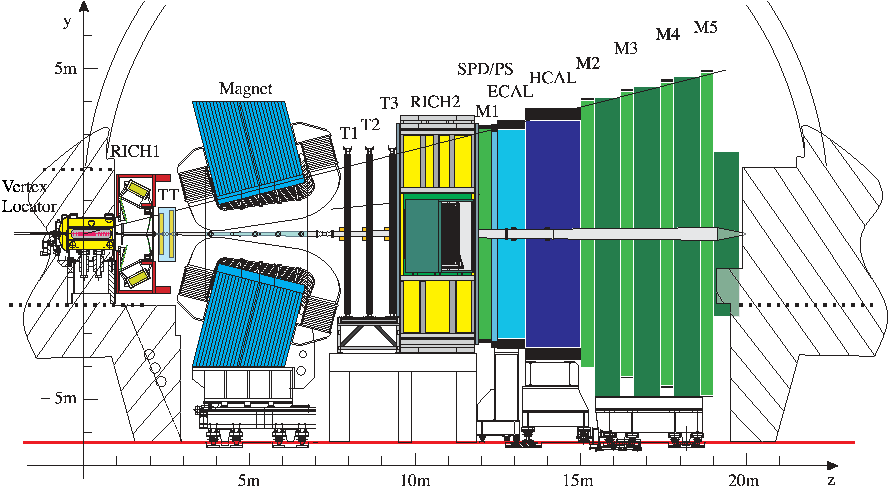
\includegraphics[width=0.8\textheight]{lhcb-detector-cross-section}
%  \caption[Cross-section view of \LHCb, cut in the non-bending $y$--$z$ plane]%
%    {Cross-section view of \LHCb, cut in the non-bending $y$--$z$ plane.}
%  \label{fig:LHCbCrossSection}
%  \end{center}
%\end{sidewaysfigure}



\chapter{Measurement of the $\nu_\mu$ charged current inclusive cross-section on Pb}
\label{chap:CrossSectionMeasurement}
This chapter presents the measurement of the $\nu_\mu$ CC inclusive cross-section on Pb using the ND280 ECals.  This chapter details the measurement method, the samples used in the measurement, the assessment of the systematic uncertainties, validation of the measurement method and finally the measurement itself.

\section{Measurement method}
\label{sec:MeasurementMethod}
The chosen method~\cite{PhysRevD.78.032003, PhysRevD.83.012005} fits a prediction to measured data using multiple data samples.  The core of the analysis method is a $\chi^2$ fit which tries to minimise the difference between the prediction and the data.  The $\chi^2$ is defined as 
\begin{equation}
  \chi^2 = \Delta \vec{N}^{\textrm{T}} \left(\underline{\underline{V}}^{\textrm{syst}} + \underline{\underline{V}}^{\textrm{stat}} \right)^{-1} \Delta \vec{N},
  \label{eqn:Chi2Def}
\end{equation}
where $\underline{\underline{V^{\textrm{syst}}}}$ and $\underline{\underline{V^{\textrm{stat}}}}$ are the systematic and statistical covariance matrices for the sample and $\Delta\vec{N}$ contains the difference between the data and the prediction for each sample.  If the number of samples used is $M$, $\Delta\vec{N}$ is defined as 
\begin{equation}
  \Delta\vec{N} = 
  \begin{pmatrix}
    N^{\textrm{data}}_1 - N^{\textrm{pred}}_1 \\
    \vdots \\
    N^{\textrm{data}}_M - N^{\textrm{pred}}_M
  \end{pmatrix}.
  \label{eqn:VecNDef}
\end{equation}
For sample $j$ of the sample set $M$, $N^{\textrm{data}}_j$ and $N^{\textrm{pred}}_j$ are the number of measured data events and number of predicted events.  The extractable information from the fit is located in $N^{\textrm{pred}}_j$ which can be subdivided into a set of templates, each of which are assigned a normalisation parameter, namely
\begin{equation}
  N^{\textrm{pred}}_j = \sum_j R_{i}n_{ij},
  \label{eqn:NPredDef}
\end{equation}
where $n_{ij}$ is the number of events in template $i$ of sample $j$ and $R_{i}$ is the normalisation assigned to that template.  The normalisation parameters are free to float in the fit and so it  is in the normisation parameters that the desired physical information is located.
\section{Input samples to the fit}
\label{sec:InputSamples}
The DS ECal provides the main signal sample which will be used to extract the cross-section.  As shown in table~\ref{table:FinalEffPur}, the selected sample in the DS ECal has the highest purity and efficiency in the whole selection making the sample the natural choice to extract the cross-section.
\newline
\newline
The method outlined above allows for the simultaneous constraint of a physical parameter and the background contamination of a set of input samples.  The method works particularly well when the input samples do not share the same sensitivity to a particular background type.  For example, in ND280, each ECal module is exposed to a different beam intensity and energy spectrum and so is exposed to a unique amount of beam induced background.  Each ECal module can be thought of as a separate input sample which fits well with the method outlined above.  So, while the DS ECal will provide the target in which the cross-section will be extracted, the barrel ECals are to also be included in the fit as a background constraint.  To further allow the barrel ECals to achieve this, an additional sample of barrel ECal events are to be included.  This additional sample set, called the 'reverse' sample set,  comes from the same data set as the selected sample described in chapter~\ref{chap:NeutrinoInteractionSelection}.  However, the events in the reverse sample set are events which pass the fiducial volume cuts but fail any other cut.  An example of a selected sample compared with a reverse sample is shown in Fig.~\ref{fig:NuEnergyReactionCodeBottomLeft}.  There are clear differences in the shape of the energy spectrum between Fig.~\ref{fig:NuEnergyReactionCodeBottomLeftSignal} and Fig.~\ref{fig:NuEnergyReactionCodeBottomLeftReverse} which suggests that the selection is biased towards lower energy neutrino interactions, despite the flat efficiency curves shown in Fig.~\ref{fig:EffPurSummedTopologiesBarrel}. The apparent bias is actually an effect of higher energy interactions creating a surplus of reconstructed events, most of which are cut away by the selection.  The shape of the true neutrino energy spectrum (see Fig.~\ref{fig:NSignalEventsTruthNeutrinoEnergy} for an example) is actually more like the selected sample shown in Fig.~\ref{fig:NuEnergyReactionCodeBottomLeftSignal}.
\begin{figure}%
  \centering
  \subfloat[Selected sample.]{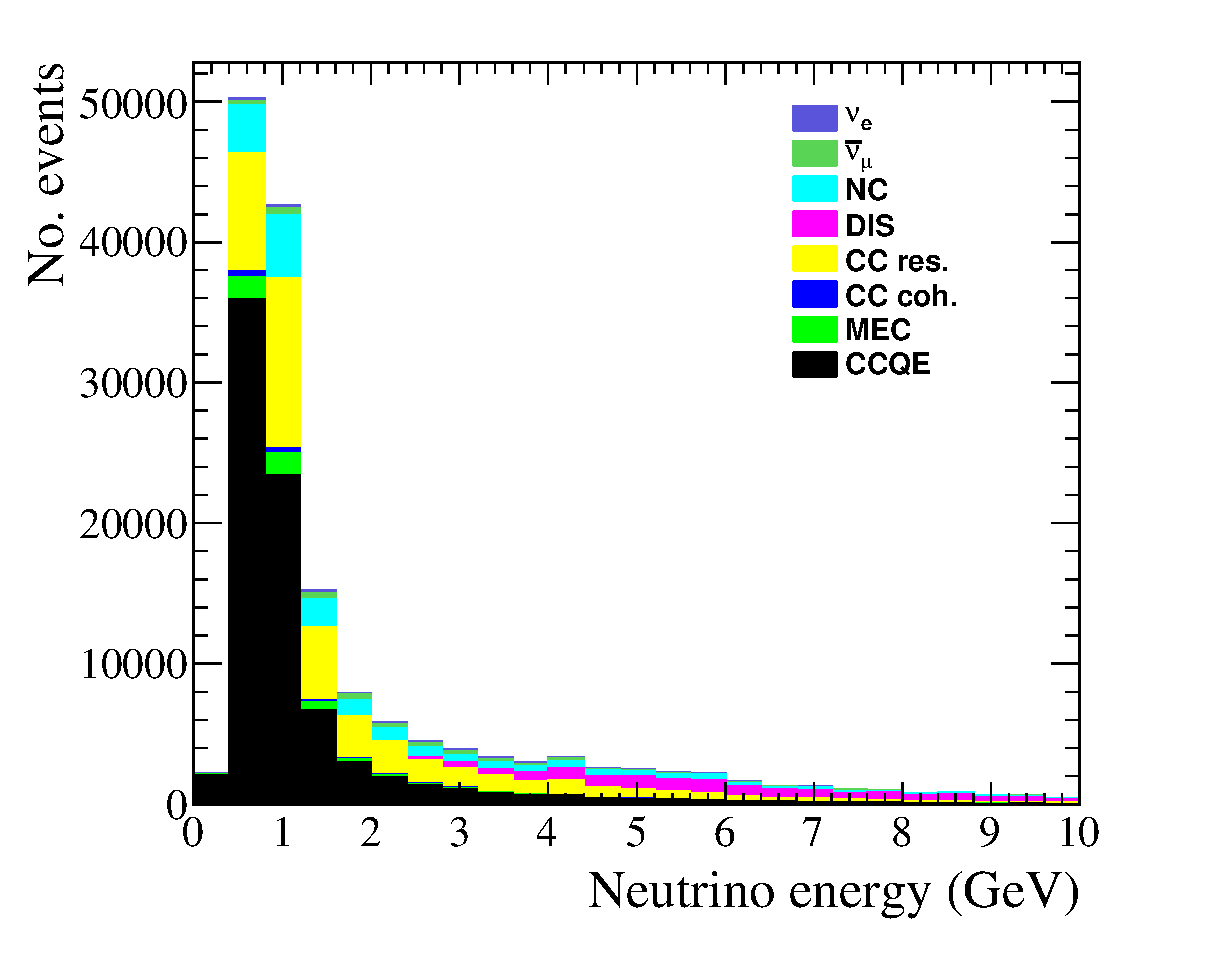
\includegraphics[width=8cm]{images/measurement/samples/NuEnergy_ReactionCode_BottomLeft_Signal.eps} \label{fig:NuEnergyReactionCodeBottomLeftSignal}}
  \subfloat[Reverse sample.]{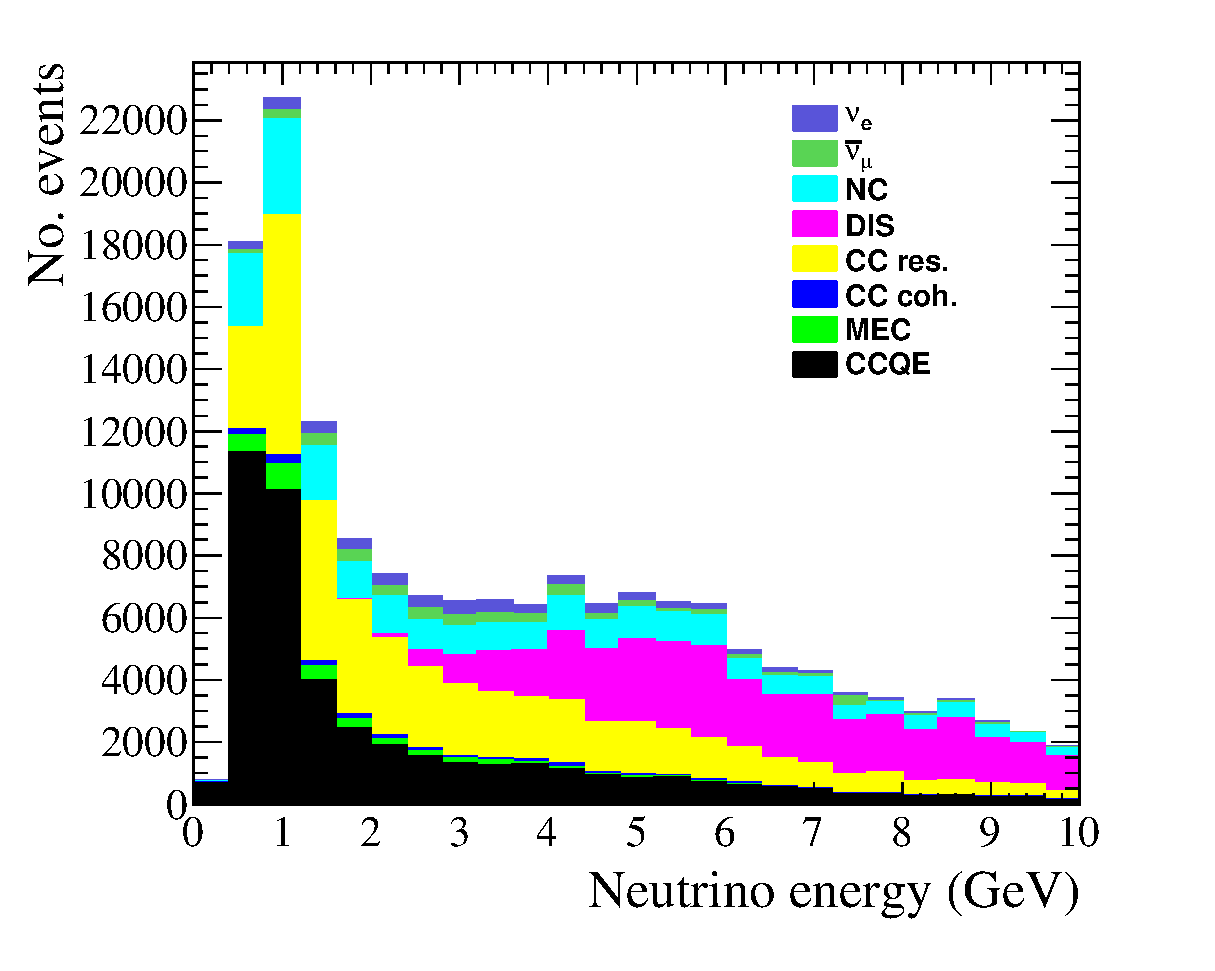
\includegraphics[width=8cm]{images/measurement/samples/NuEnergy_ReactionCode_BottomLeft_Reverse.eps} \label{fig:NuEnergyReactionCodeBottomLeftReverse}}
  \caption{The neutrino energy of events seen in the bottom-left ECal module broken down by the neutrino interaction mode.}
  \label{fig:NuEnergyReactionCodeBottomLeft}
\end{figure}
\newline
\newline
As described in chapter~\ref{chap:NeutrinoInteractionSelection}, the developed selection does not distinguish between lead and carbon interactions, partly because such events are indistinguishable from one another.  It is however desirable to separate the two catagories out as the presented measurement purely involves lead.  As the ECal is not capable of separating the events by itself, an additional constraint is needed.  So, a sample of CC interactions on carbon occurring in the FGD are also included, which are taken from the official ND280 oscillation input analysis [INSERT TECHNOET REFERENCE!!!!!].
\newline
\newline
To summarise, there are many inputs samples to the measurement.  Specifically, there are 12 barrel ECal samples (6 selected and 6 reverse), the DS ECal sample and the FGD sample which totals to 12 input samples.

\section{The ECal rate fit}
\label{sec:ECalRateFit}
Now that the general method and the input samples have been introduced, the fit used by the analysis can be introduced.  The fit itself is a data-driven constraint of the event rate in each ECal module where the Monte Carlo prediction is separated into templates whose normalisation is allowed to vary.  The machinery outlined in section~\ref{sec:MeasurementMethod} almost completely decribes what is required to understand the fit, however two specific definitions are needed.  The first is that there are 12 input samples to the fit.  The second is the definition of $N^{\textrm{pred}}_i$.  To constrain the lead event rate, three Monte Carlo templates are needed: a lead template which contains any reconstructed event associated with a $\nu_\mu$ CC interaction on lead, a carbon template which contains any reconstructed event associated with a $\nu\mu$ CC interaction on carbon and an 'other' template which contains any reconstructed event which does not fall into the above two catagories.  $N^{\textrm{pred}}_i$ is then defined as 
\begin{equation}
  N^{\textrm{pred}}_i = R^{\textrm{Pb}}n^{\textrm{Pb}}_i + R^{\textrm{C}}n^{\textrm{C}}_i + R^{\textrm{other}}n^{\textrm{other}}_i,
  \label{eqn:ECalFitPredDef}
\end{equation}
where $n^{\textrm{X}}_i$ is the number of events in template X of sample $i$ and $R^{\textrm{X}}_i$ is the variable normalisation of that template.
\newline
\newline
The rate fit allows $R^{\textrm{Pb}}_i$, $R^{\textrm{C}}_i$ and $R^{\textrm{oth}}_i$ to vary with no prior constraint in an attempt to minimise the $chi^{2}$ as defined in equation~\ref{eqn:Chi2Def}.  Once the minimum has been found, the fitted $R^{\textrm{Pb}}_i$ can then be used to extract the cross-section using the selected events in the DS ECal.  
\newline
\newline
The number of events in each input sample, broken down by the template contribution, is shown in Fig.~\ref{fig:NominalMCTemplates}.  As should be expected, the relative backround contribution varies between each ECal module.
\begin{figure}
  \centering
  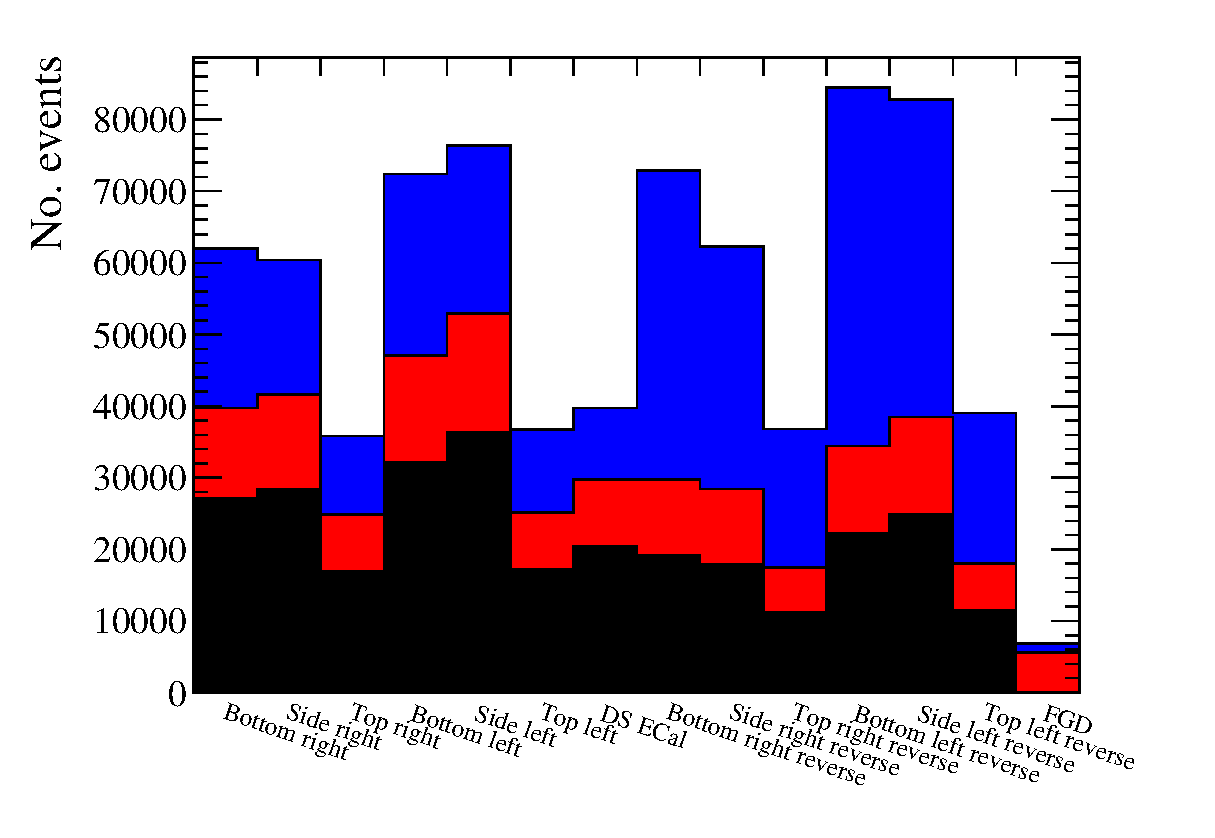
\includegraphics[width=15cm]{images/measurement/rate_fit/MC_Templates_Nominal.eps}
  \caption{The number of events in each input sample separated into the lead (black), carbon (red) and other (blue) templates.}
  \label{fig:NominalMCTemplates}
\end{figure}
\newline
\newline
The underlying fit machinery uses the Minuit2 algorithm provided by the ROOT TFitter framework, chosen primarily because of its ease of use.


\section{Systematic uncertainties}
\label{sec:SystematicUncertainties}
The $\chi^2$ definition shown in equation~\ref{eqn:Chi2Def} allows for systematic uncertainties to be directly included in the fit.  As the systematic uncertainty implementation takes the form of a covariance matrix for the input samples, a good understanding of not only the systematic uncertainties, but how the samples correlate with one another is needed.  
\newline
\newline
As stated above, there are 12 input samples so the covariance matrix will be a 12$\times$12 symmetric matrix.  While it may be obvious that the contents of the matrix will be the covariances of each input sample, it may not be immediately clear what type of covariances are needed.  As described in section~\ref{sec:ECalRateFit}, the algorithm attempts to fit a set of predictions, separated into templates, to a set of measured data samples simultaneously.  The variation comes from the normalisations assigned to each template.  This means that the overall normalisation of the Monte Carlo prediction is free to vary without prior constraint and so it is the shape information between the prediction and data that constrains the parameters.  Therefore the covariance matrix used in the fit should only contain uncertainties which account for the differences in the shape of the samples which the systematic sources introduce.
\newline
\newline
The ND280 event simulation is essentially broken down into three areas: Simulation of the neutrino flux, simulation of the neutrino interactions and simulation of the detector response.  No matter how complicated a simulation can become, it is unlikely to ever simulate reality with $100\%$ accuracy.  The differences between what is simulated (be it flux, interaction or detector) and what happens in nature causes a systematic difference to be seen between collected data and Monte Carlo which must be accounted for.  As the simulation can be broken down into three key areas, the systematic assessment can be broken down into the same key areas, each of which are presented.  The actual assessment of a systematic uncertainty can be broken down into two areas: identifaction of a systematic error source and the propagation of that systematic error source through the analysis.  The identification stage is typically handled by a respective working group or by an analyser with external sources (e.g. control samples).  The propagation of the systematic error source has no strict recipe but it typically involves variation of the identified systematic uncertainty and then either a reweighting of events is applied or the analysis chain is re-run.  The systematic treatment used in this analysis uses a mixture of the above.
\newline
\newline
To propagate the systematic uncertainty effect, a Monte Carlo sample akin to the prediction sample set used in the fit is required.  So, a $2.5\times10^{19}$ POT sub sample of beam and sand Monte Carlo is used for this purpose.  All sample systematic covariance matrices are presented as fractional covariance matrices between each of the different detector samples.  For the barrel samples, the selected samples are labelled by their respective module name and the reverse barrel samples (background enriched samples) are labelled with their module name and 'reverse'.  The assessment of each systematic source is presented individually, resulting in a fractional covariance matrix for that source.  The final systematic covariance matrix is then found by summing all of the individual covariance matrices.
\subsection{Flux systematic evaluation}
\label{subsec:FluxSystematic}
The neutrino flux is one of the core components of the ND280 event simulation and any uncertainties associated with the flux have a direct impact on the measured ND280 event rate.  The associated flux uncertainties can be broken down into four catagories:
\begin{itemize}
  \item Properties of the proton beam such as profile and alignment
  \item Alignment of the target and focusing horns
  \item The current in the focusing horns and the magnetic field it generates
  \item Hadron production induced by beam interactions with the target
\end{itemize}
As the neutrino flux prediction is so important for all T2K analyses, the flux uncertainties are constrained using a range of measurements.  These include external measurements from the NA61/SHINE collaboration, from the proton beam monitors, measurements of a spare magnetic horn and from the INGRID detector.  Measured uncertainties from each source are used to vary the flux in JNUBEAM which produces a covariance matrix for each source.  The covariance matrix then used by analyser is the sum of each covariance matrix which is shown in Fig.~\ref{fig:FluxPredictionSyst}.  The covariance matrix is split into two detector sections: ND280 and SK.  Each detector section is then separated into two beam running modes ($\nu$ and $\bar{\nu}$ runnings) which are also separated into four neutrino flavours ($\nu_\mu$, $\bar{\nu}_\mu$, $\nu_e$ and $\bar{\nu}_e$).  Finally, each neutrino flavour is separated into a set of energy bins.  The presented analysis is a $\nu_\mu$ cross-section measurement using ND280, so only the ND280, $\nu$-running mode section of the covariance matrix needs consideration.
\begin{figure}
  \centering
  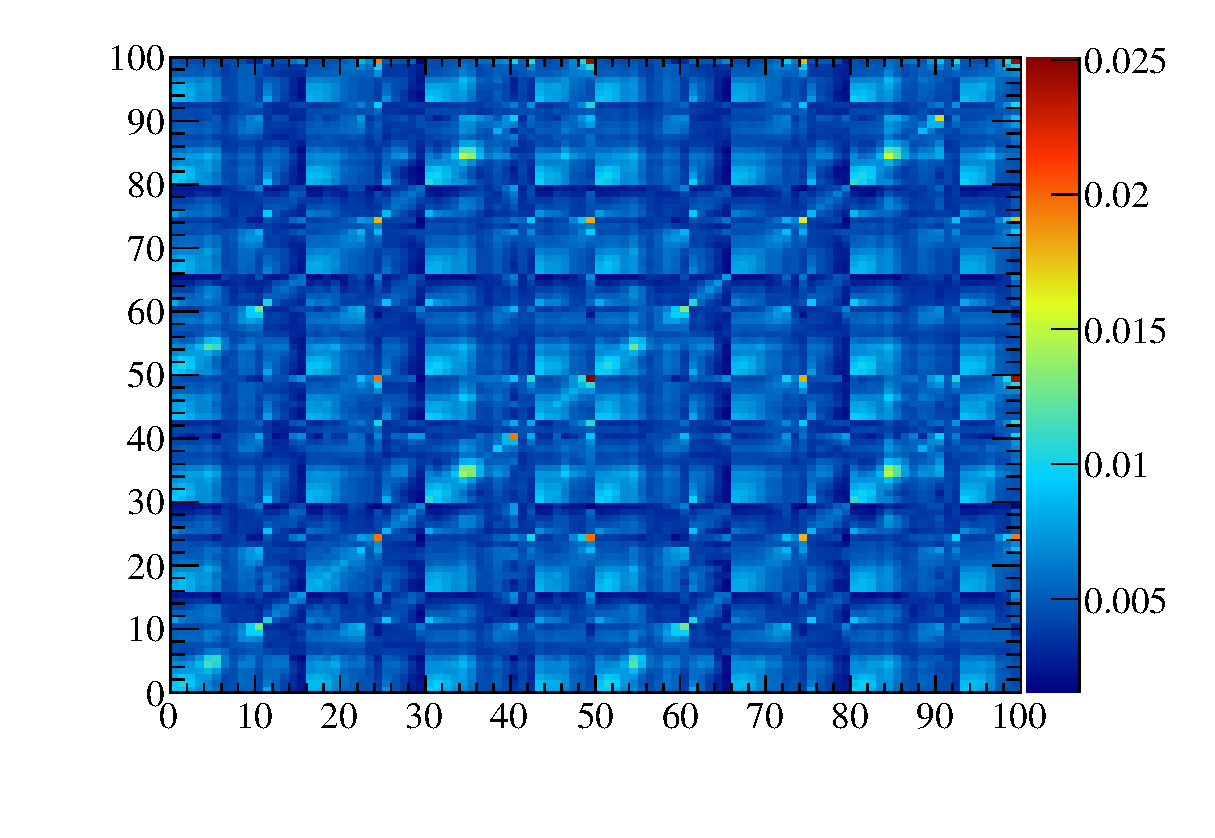
\includegraphics[width=12cm]{images/measurement/systematics/flux/flux_prediction_syst.eps}
  \caption{The flux prediction covariance matrix.  The matrix is binned in detector (SK and ND280), neutrino flavour and energy.}
  \label{fig:FluxPredictionSyst}
\end{figure}
The provided flux covariance matrix is a fractional covariance matrix, binned in netrino energy and flavour.  As the neutrino energy and flavour information of events seen in this analysis is readily available, the flux covariance matrix can be used to reweight the events in the Monte Carlo sample to propagate the effect of the systematic uncertainty through the analysis.  To do this, the flux covariance matrix is Cholesky decomposed and the resulting matrix multiplied by a vector filled with random throws from a Gaussian of mean 0 and width 1.  Each element in this multiplied vector constitutes a fractional change in the number of a specific neutrino flavour and energy seen in the analysis.  So, the event weightings are generated by adding 1 to each element of this vector.  Every event selected in the sample is then weighted by the correct event weight (in this case defined by the neutrino flavour and energy) and this number of reweighted events is then recorded.  The above description describes a single throw of the flux systematic propagation.  This process is repeated 1000 times to build up the covariance matrix for the sample.  The sample covariance matrix elements are calculated as
\begin{equation}
  V_{\textrm{ab}} = \frac{1}{N^{\textrm{throws}}}\sum^{N^{\textrm{throws}}}_{i=1}\frac{\left(N_{\textrm{a}}^{i} - N_{\textrm{a}}^{\textrm{nom}}\right)\left(N_{\textrm{b}}^{i} - N_{\textrm{b}}^{\textrm{nom}}\right)}{N_{\textrm{a}}^{\textrm{nom}}N_{\textrm{b}}^{\textrm{nom}}},
  \label{eqn:CovarianceMatrixElementDef}
\end{equation}
where $N_{\textrm{a}}^{\textrm{nom}}$ is the number of events seen in the nominal Monte Carlo for sample a and $N^{\textrm{throws}}$. $N_{\textrm{a}}^{i}$ is generically the number of events seen in sample a for systematic throw $i$, but its definition depends on which kind of covariance matrix is being calculated.  For a shape+normalisation covariance matrix, $N_{\textrm{a}}^{i}$ is defined as 
\begin{equation}
  N_{\textrm{a}}^{i} = N^{i\prime}_{\textrm{a}}, 
  \label{eqn:NVariedDef}
\end{equation}
where $N^{i\prime}_{\textrm{a}}$ is simply the number of events in sample a for throw $i$ after applying the systematic variation.  In the above example, this after applying the event reweighting based on the flux covariance matrix.  When considering a shape-only covariance matrix, $N_{\textrm{a}}^{i}$ is 
\begin{equation}
  N_{\textrm{a}}^{i} = N^{i\prime}_{\textrm{a}}\frac{\displaystyle\sum_{j=1}^{12}N_{\textrm{j}}^{\textrm{nom}}}{\displaystyle\sum_{j=1}^{12}N^{i\prime}_{\textrm{j}}}. 
  \label{eqn:NVariedShapeOnlyDef}
\end{equation}
The extra factor on the RHS of equation~\ref{eqn:NVariedShapeOnlyDef} convserves the total number of events seen such that there are an equal total number of events before and after applying the systematic variation.  The sample covariance matrices found by applying the above process are shown in Fig.~\ref{fig:FluxCovarianceMatrices}.
\begin{figure}%
  \centering
  \subfloat[Shape+normalisation.]{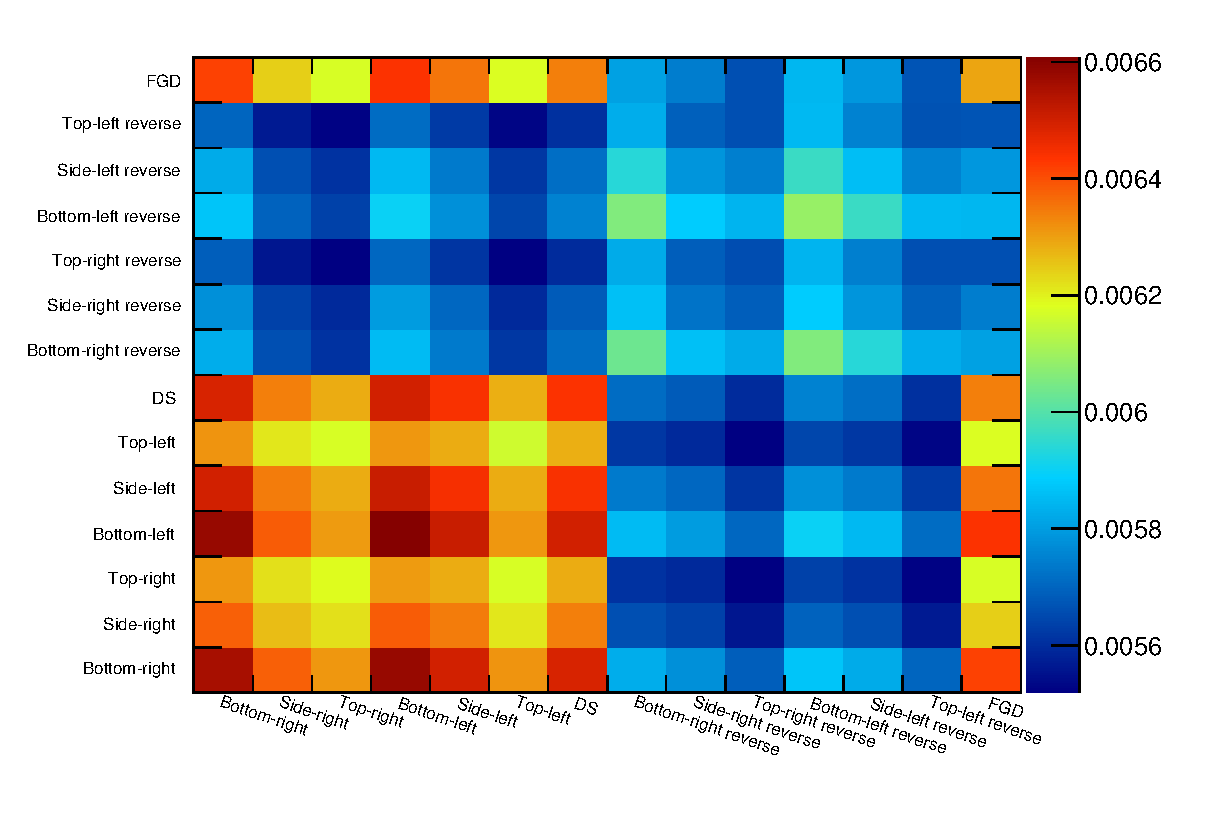
\includegraphics[width=8cm]{images/measurement/systematics/flux/flux_covariance_matrix.eps} \label{fig:FluxShapeNormCovarianceMatrix}}
  \subfloat[Shape-only.]{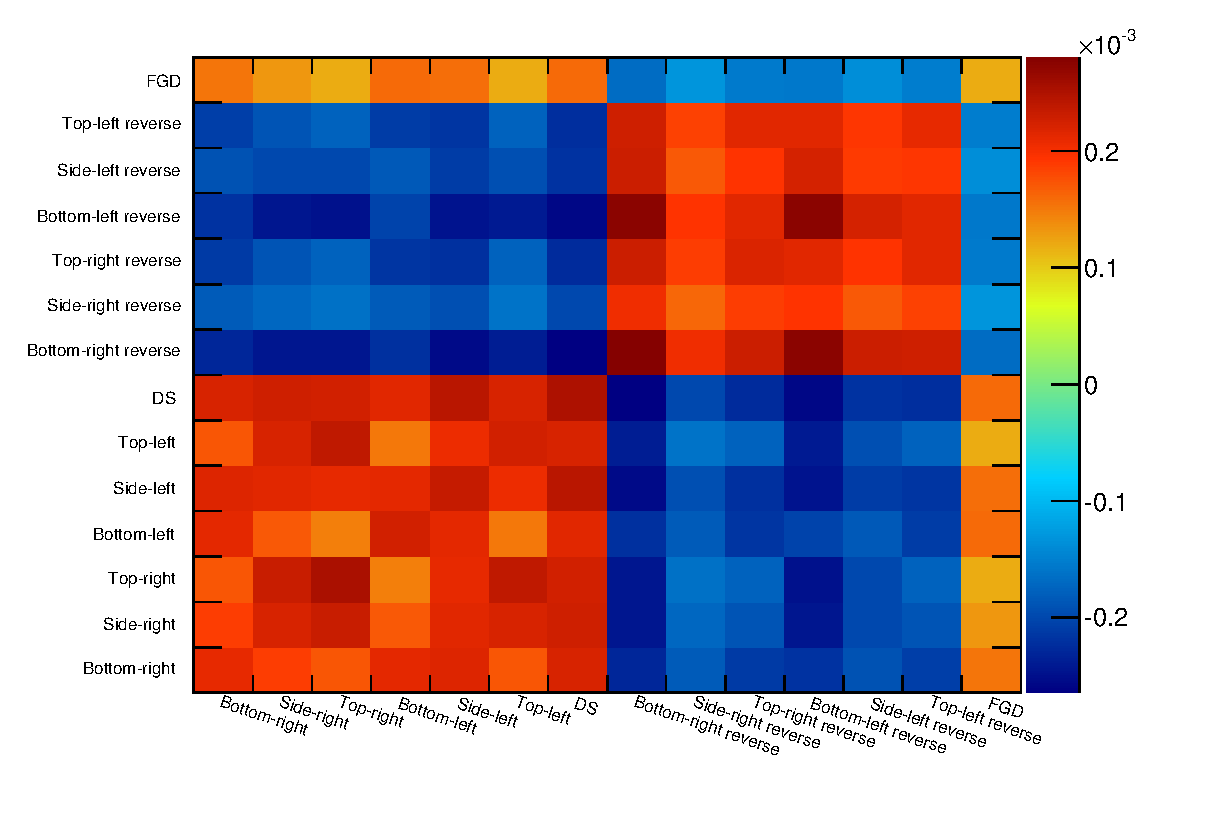
\includegraphics[width=8cm]{images/measurement/systematics/flux/flux_shape_covariance_matrix.eps} \label{fig:FluxShapeOnlyCovarianceMatrix}}
  \caption{The sample covariance induced by the flux uncertainties.}
  \label{fig:FluxCovarianceMatrices}
\end{figure}
\newline
\newline
The effect of the flux systematic on the selection efficiency of lead interactions was also evaluated.  As the main target used in this analysis is the DS ECal, the efficiency variation was evaluated for this detector only.  For each systematic throw described above, the selection efficiency was calculated and recorded.  By plotting the efficiency for each throw, the width of the efficiency distribution can be found which gives the efficiency uncertainty induced by the flux systematic.  This efficiency uncertainty was found to be 0.00097.  The lead selection efficiency in the DS ECal is nominally 0.539, which implies a fractional change of 0.18$\%$, which is essentially negligable.
\begin{figure}
  \centering
  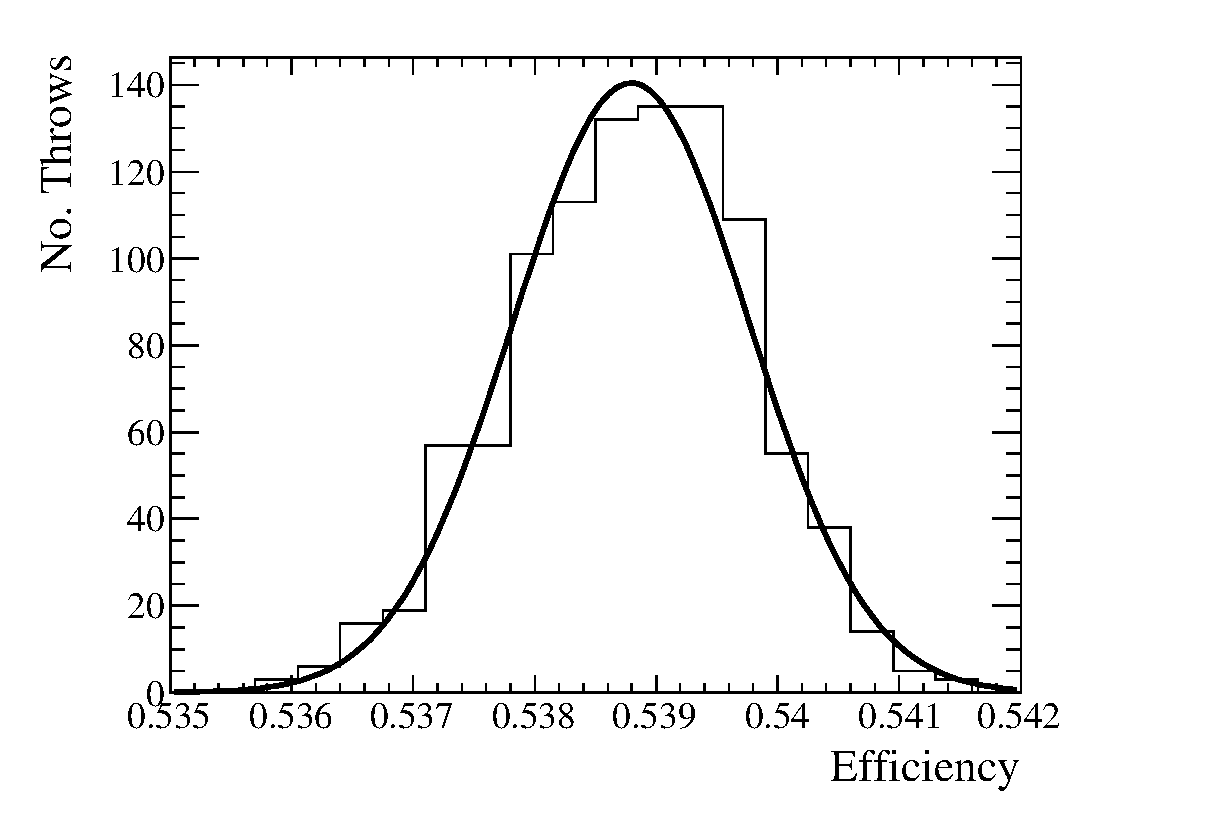
\includegraphics[width=12cm]{images/measurement/systematics/flux/flux_efficiency_variation.eps}
  \caption{The variation in the selection efficiency of lead interactions in the DS ECal caused by the flux systematic.}
  \label{fig:FluxEfficiencyVariation}
\end{figure}
\subsection{Cross-section systematic evaluation}
\label{subsec:CrossSectionSystematic}
The neutrino cross-section picture is still a very much open area of research.  The interaction model used by current neutrino interaction generaters use a set of empirical parameters which are tuned on experimental results.  Uncertainties on any one of these empirical parameters will alter the simulated cross-section and thus the event rate seen in the ND280 simulation.  A dedicated working group handles the assessment of the empirical parameters and their corresponding uncertainties.  The parameter uncertainties are given as a covariance matrix along with the known correlations which is shown in Fig.~\ref{fig:XSecPredictionSyst}.  The interaction parameter assessment is chiefly undertaken with the T2K oscillation analyses in mind which means that the nuclear model parameters are only considered for carbon and oxygen.  In the presented analysis, iron and aluminium are two major sources of background interactions which must also be treated in the systematic assessment.  The chosen treatment is to assign a data-motivated, normalisation uncertainty to such backgrounds.  The iron uncertainty is taken from the iron cross-section measurement using INGRID.  The aluminium uncertainity is taken from [INSERT DETAILS HERE].  As element specific parameters for lead do not appear in Fig.~\ref{fig:XSecPredictionSyst}, such parameters are additionally assessed separately using NEUT.
\begin{figure}
  \centering
  %INSERT XSEC COVARIANCE MATRIX
  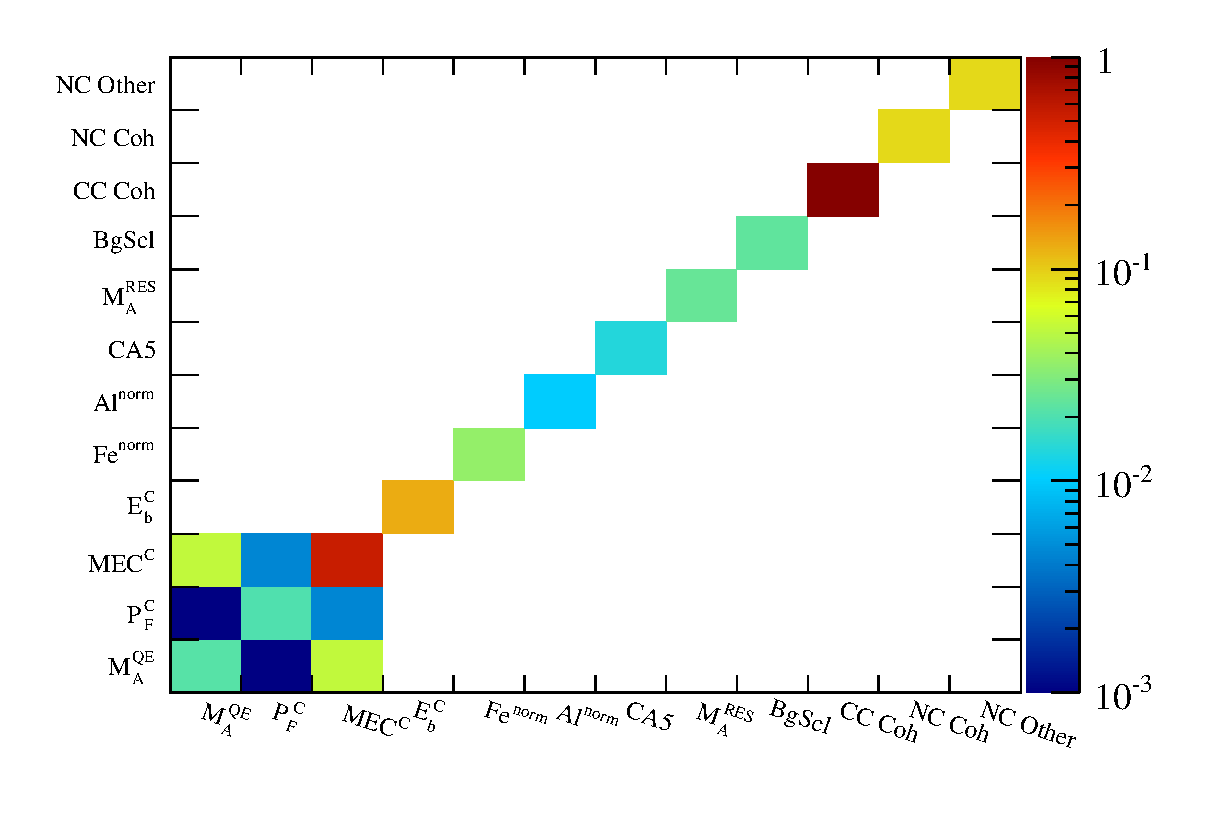
\includegraphics[width=12cm]{images/measurement/systematics/xsec/xsec_prediction_syst.eps}
  \caption{The neutrino cross-section model covariance matrix.}
  \label{fig:XSecPredictionSyst}
\end{figure}
\newline
\newline
To propagate the effect of the cross-section systematic through the analysis, the covariance matrix shown in Fig.~\ref{fig:XSecPredictionSyst} was Cholesky decomposed and the resultant matrix multiplied by a vector of random numbers thrown from a gaussian (the same approach as described in section~\ref{subsec:FluxSystematic}).  However, the re-weighting in this case is more complicated.  The T2KReWeight [INSERT REFERECE] software takes the parameters errors from the throw along with the simulated NEUT vertex which is matched to the event.  T2KReWeight then calculates a weight based on the inputted errors and the NEUT vertex in question.  Using the T2KReWeight machinery, 1000 systematic throws from the covariance matrix shown in Fig.~\ref{fig:XSecPredictionSyst} were made and sample covariance matrices were calculated, which are shown in Fig.~\ref{fig:XSecCovarianceMatrices}.
\begin{figure}%
  \centering
  \subfloat[Shape+normalisation.]{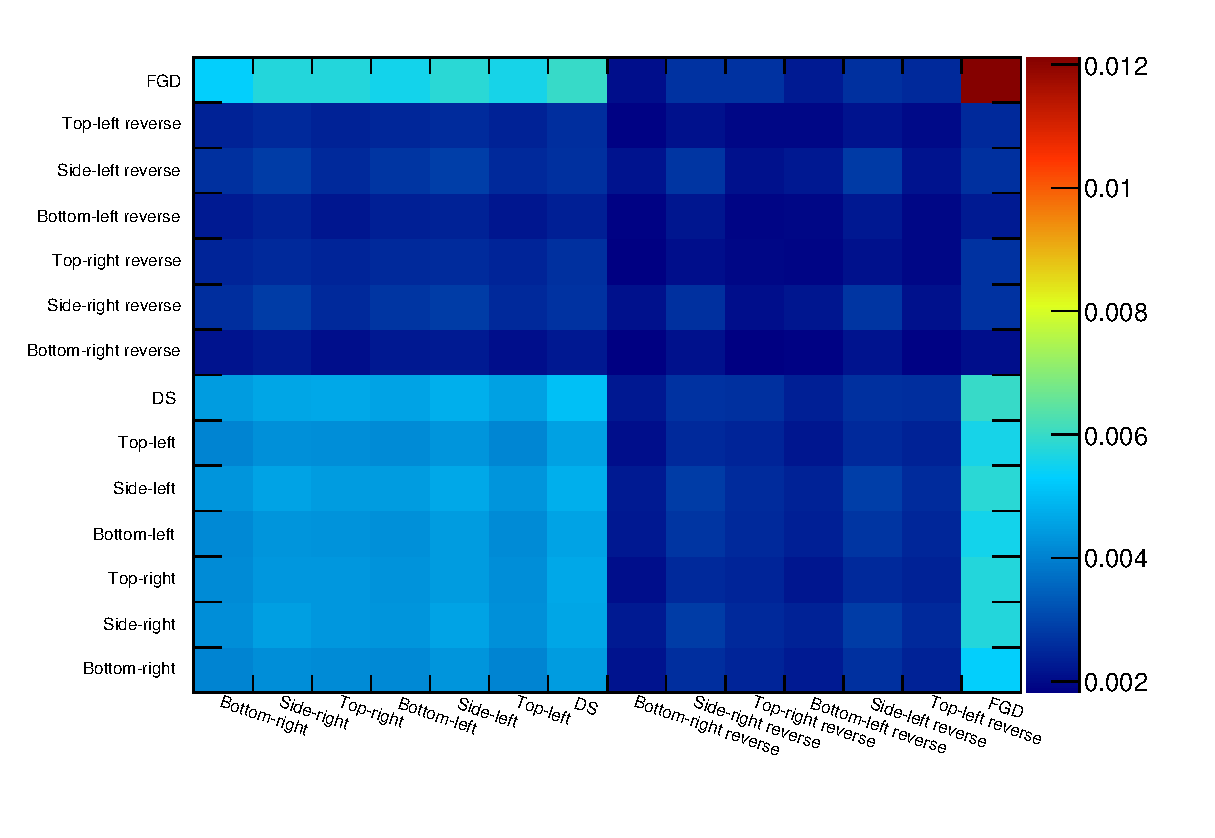
\includegraphics[width=8cm]{images/measurement/systematics/xsec/xsec_covariance_matrix.eps} \label{fig:XSecShapeNormCovarianceMatrix}}
  \subfloat[Shape-only.]{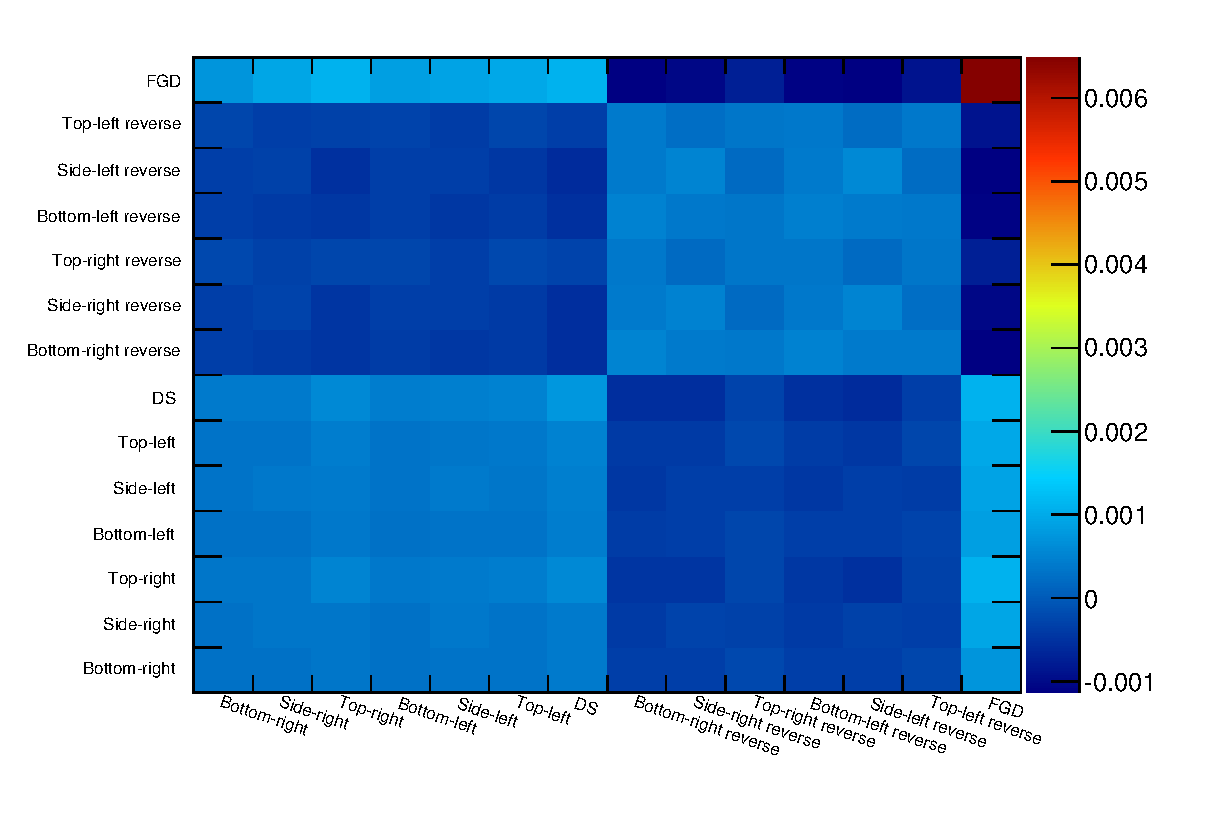
\includegraphics[width=8cm]{images/measurement/systematics/xsec/xsec_shape_covariance_matrix.eps} \label{fig:XSecShapeOnlyCovarianceMatrix}}
  \caption{The sample covariance induced by the cross-section model uncertainties.}
  \label{fig:XSecCovarianceMatrices}
\end{figure}
\newline
\newline
As with the flux systematic, the uncertainty in the selection efficiency for lead interactions in the DS ECal due to the cross-section model systematic was found by recording the efficiency for each throw.  The variation in the efficiency is shown in Fig.~\ref{fig:XSecEfficiencyVariation}.  The efficiency uncertainty was found to be 0.001 which corresponds to a 0.2$\%$ error which is, again, negligable.
\begin{figure}
  \centering
  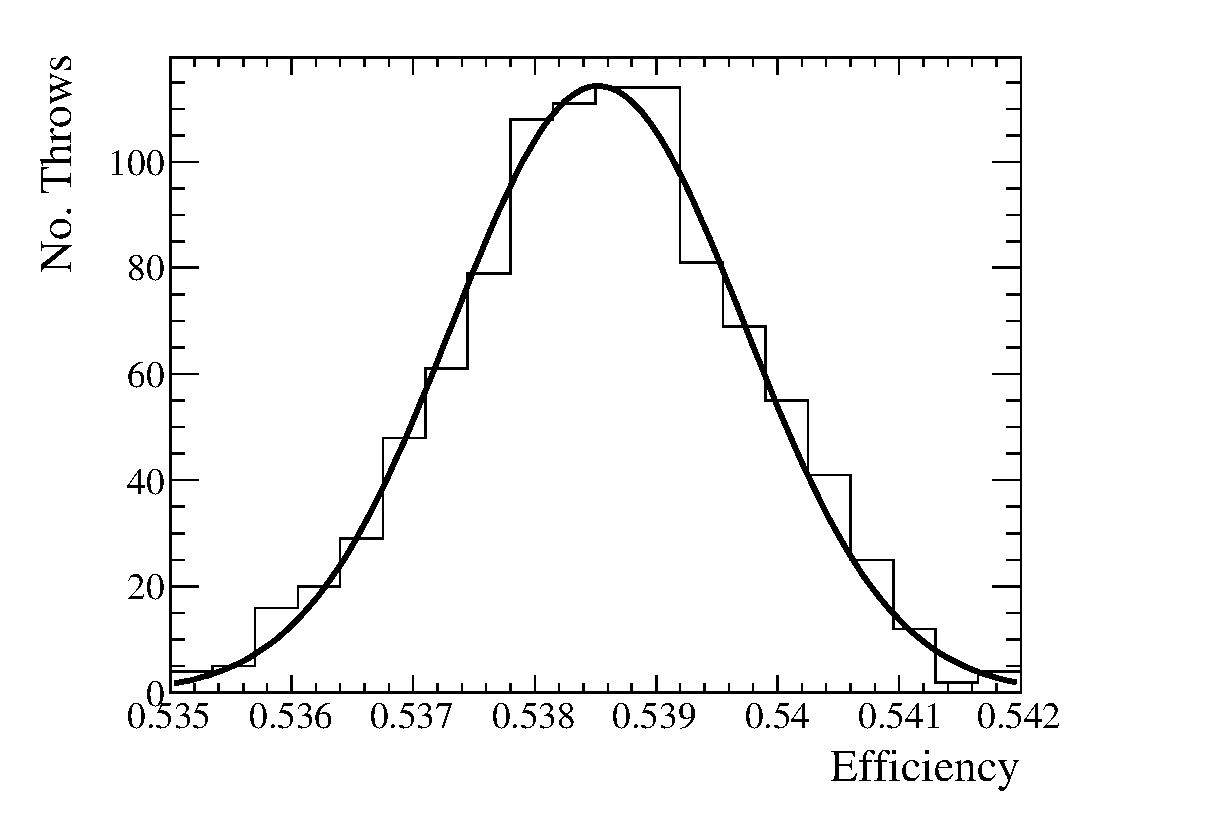
\includegraphics[width=12cm]{images/measurement/systematics/xsec/xsec_efficiency_variation.eps}
  \caption{The variation in the selection efficiency of lead interactions in the DS ECal caused by the cross-section model systematic.}
  \label{fig:XSecEfficiencyVariation}
\end{figure}
\newline
\newline
As discussed above, the re-weighting of element specific parameters for events matched to a lead interactions was not possible using T2KReWeight.  As meson-exchange current interactions for lead interactions are not implemented in NEUT, the only parameters necessary to vary are $P_{\textrm{F}}^{\textrm{Pb}}$ and $E_{\textrm{b}}^{\textrm{Pb}}$ which are the Fermi-momentum and binding energy for lead respectively.  So, NEUT was used to produce 10,000 neutrino interactions on lead with uniform energy between 0~GeV and 10~GeV for the nominal parameters and $\pm\upsigma$ variations of the parameters.  The associated uncertainties were not readily available in the literature so $1.5\times$ the carbon parameters uncertainties were used as a conservative estimate.  The NEUT events were used to plot the ratio of the varied cross-section to the nominal cross-section as a function of energy.  The ratios for $P_{\textrm{F}}^{\textrm{Pb}}$ and $E_{\textrm{b}}^{\textrm{Pb}}$ are shown in Fig.~\ref{fig:PbXSecPfRatio} and Fig.~\ref{fig:PbXSecEbRatio} respectively.  The variation in the cross-section caused by variation in $E_{\textrm{b}}^{\textrm{Pb}}$ is sub-percent so there should be a negligable variation in the event rate which means this can be ignored.  However, there is significant variation in the cross-section at low energy due to variations in $P_{\textrm{F}}^{\textrm{Pb}}$ so this effect must be propgated through the analysis.  To do this, the ratio distributions shown in Fig.~\ref{fig:PbXSecPfRatio} were treated as a set of events weights.  The $+\upsigma$ and $-\upsigma$ weights were applied to the sample separately, creating two systematics throws.  The results of the systematic throws were used to generate the sample covariances, which are shown in Fig.~\ref{fig:PbXSecCovarianceMatrices}.
\begin{figure}%
  \centering
  \subfloat[$P_{\textrm{F}}^{\textrm{Pb}}$]{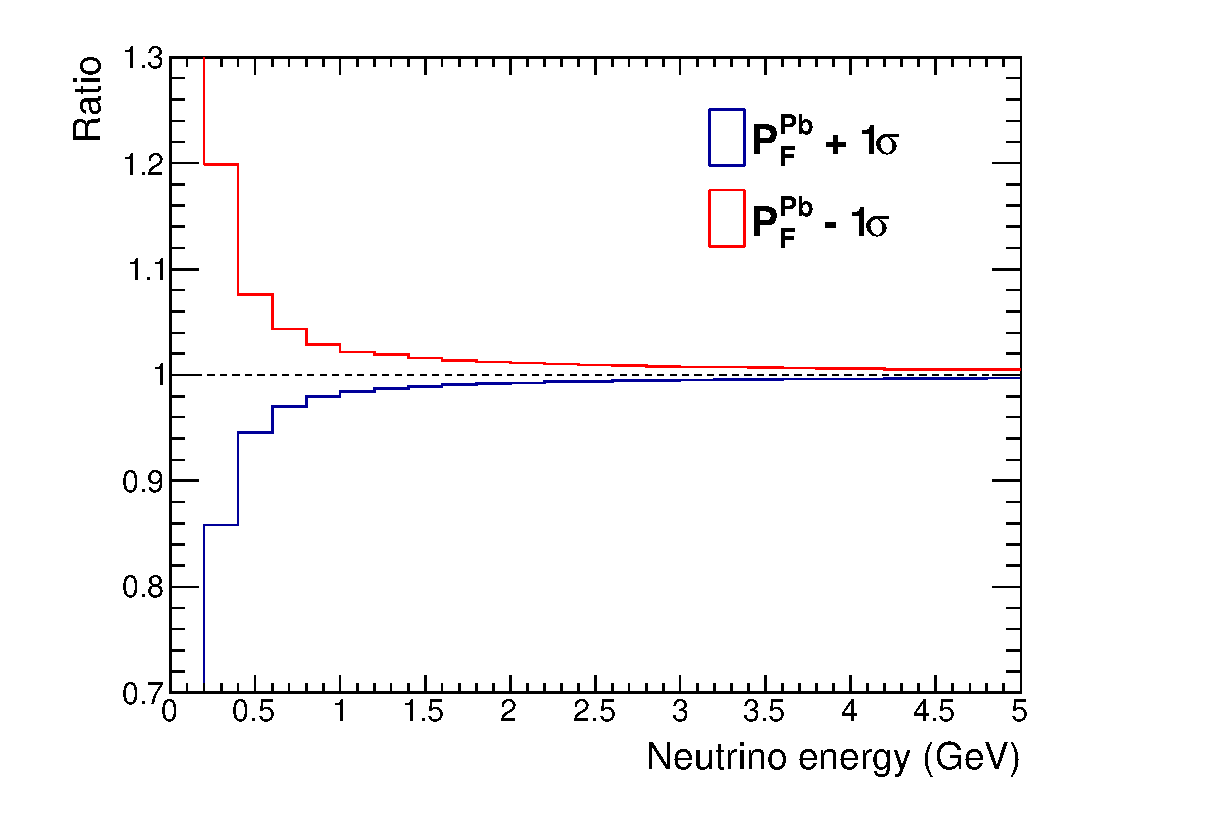
\includegraphics[width=8cm]{images/measurement/systematics/xsec/pbxsec_pf_ratio.eps} \label{fig:PbXSecPfRatio}}
  \subfloat[$E_{\textrm{b}}^{\textrm{Pb}}$]{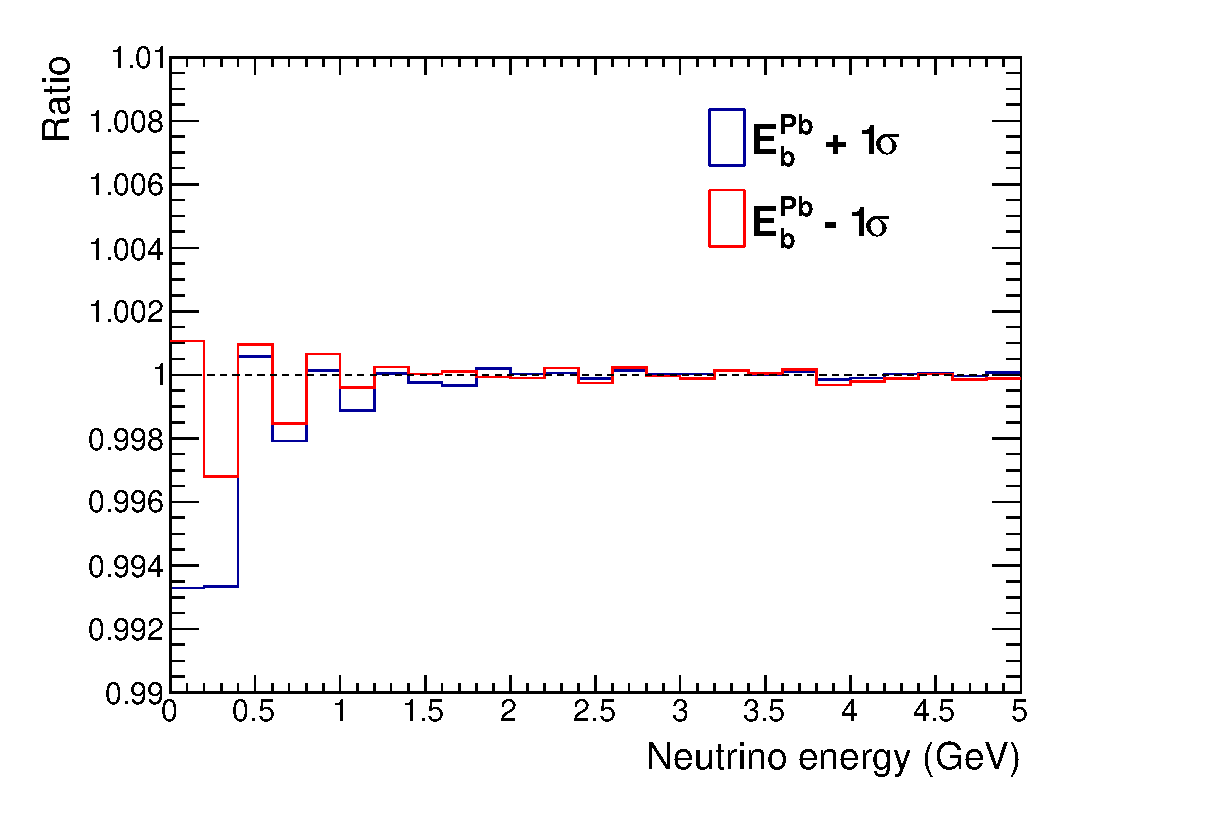
\includegraphics[width=8cm]{images/measurement/systematics/xsec/pbxsec_eb_ratio.eps} \label{fig:PbXSecEbRatio}}
  \caption{The ratio of the $\pm$$\upsigma$ cross-section to the nominal cross-section for lead as a function of neutrino energy.}
  \label{fig:PbXSecRatios}
\end{figure}
\begin{figure}%
  \centering
  \subfloat[Shape+normalisation.]{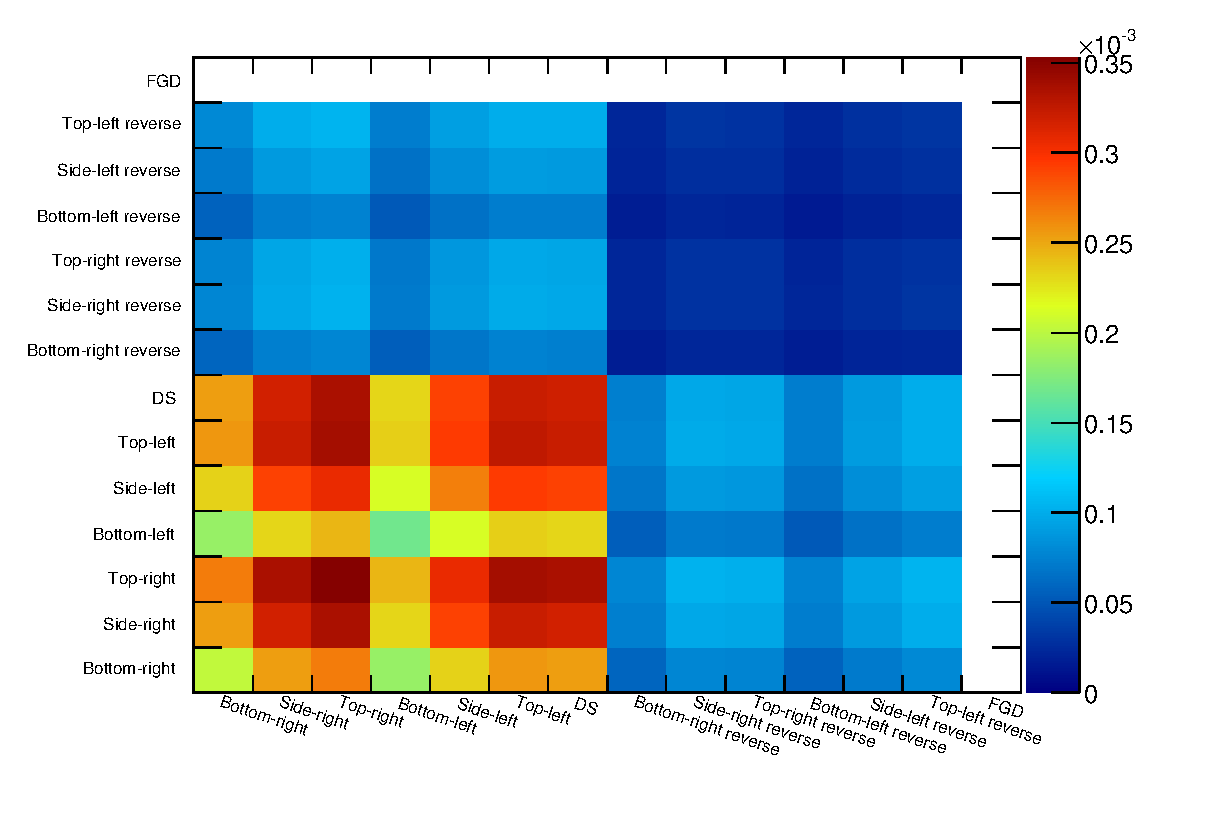
\includegraphics[width=8cm]{images/measurement/systematics/xsec/pb_xsec_covariance_matrix.eps} \label{fig:PbXSecShapeNormCovarianceMatrix}}
  \subfloat[Shape-only.]{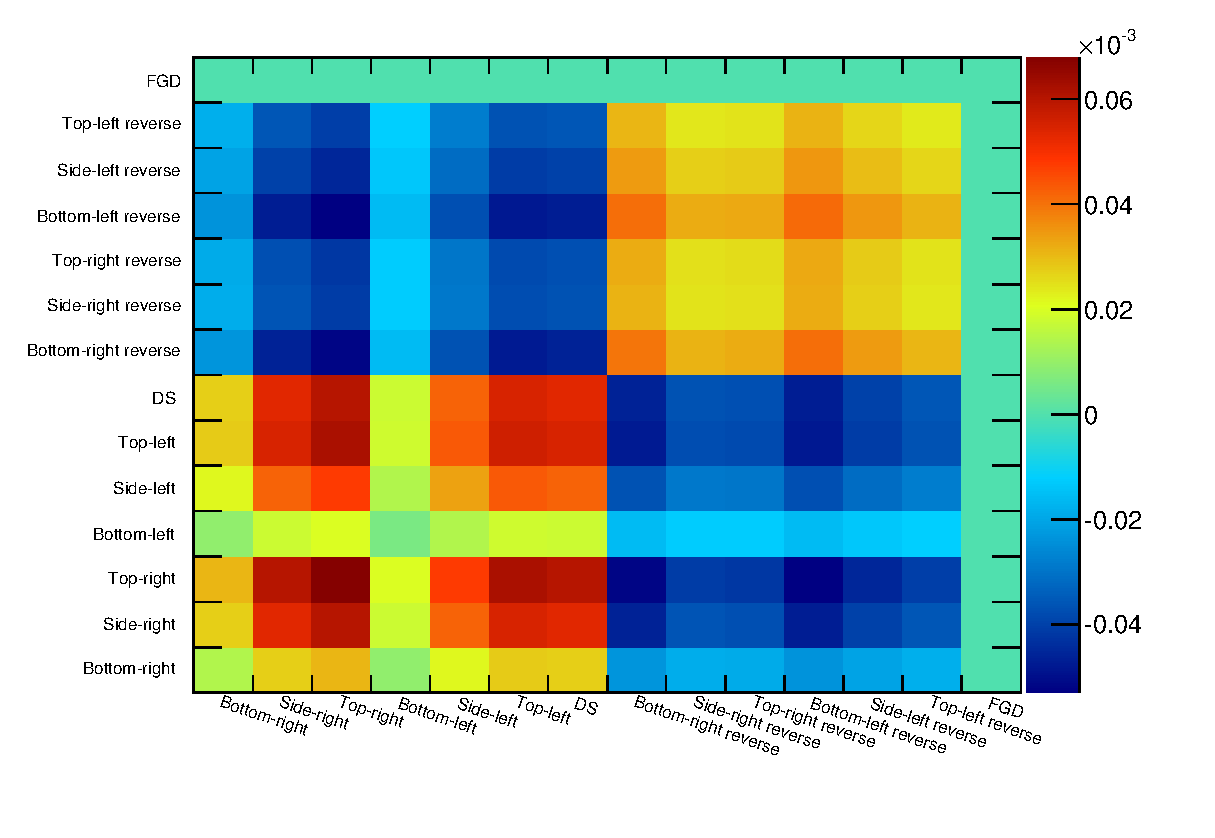
\includegraphics[width=8cm]{images/measurement/systematics/xsec/pb_xsec_shape_covariance_matrix.eps} \label{fig:PbXSecShapeOnlyCovarianceMatrix}}
  \caption{The sample covariance induced by variation of $P_{\textrm{F}}^{\textrm{Pb}}$.}
  \label{fig:PbXSecCovarianceMatrices}
\end{figure}
\newline
\newline
Final state interactions (FSI) within the nucleus after a neutrino interaction has occurred could also cause a variation in the event rate.  While the selection used in this analysis is CC inclusive, the method used separates events out into prong topologies.  Any uncertainty in the FSI could cause migration of events from one prong topology to another.  The Neutrino Interaction Working Group (NIWG) assesses these uncertainties and provides a set of parameters for an analyser to vary, all of which are associated with $\pi^{\pm}$ interactions.  There are six parameters associated with FSI:
\begin{itemize}
  \item Low energy quasi-elastic scattering (FSIQEL)
  \item High energy quasi-elastic scattering (FSIQEH)
  \item Pion production (FSIINEL)
  \item Pion absorption (FSIABS)
  \item Low energy single charge exchange (FSICXL)
  \item High energy single charge exchange (FSICXH)
\end{itemize}
The NIWG provides combinations of the $1\upsigma$ errors for the parameters highlighted above which span the whole FSI parameter space.  The errors are provided in 16 parameters sets which represent the $1\upsigma$ contour for the FSI parameter space and are shown in table~\ref{table:FSIErrors}.  Each parameter set can be used to generate one systematic throw, by passing the parameters to T2KReWeight and subsequently re-weighting the events.  As with the cross-section model systematics described above, the parameter variations only affect carbon and oxygen.  The FSI systematic throws were used to generate the sample covariance matrices which are shown in Fig.~\ref{fig:FSICovarianceMatrices}.
%\newline
%\newline
%It is not trivial how to assess how the FSI uncertainties affect the lead interactions as the T2KReWeight machinery can not be used.  FSI should cause a mixing between the different CC interaction final states which means that there will be migration from one prong topology to another.  Based on the efficiencies in table~\ref{table:SelEfficiency}, the main concern would be from 2 prong topology events migrating to 1 prong topology events in the barrel where such events would be exposed to a stream of cuts which are 12$\%$ less efficient.  Assuming that the variation in event rate induced by the FSI variation for carbon/oxygen is similar for lead, the change in events seen would be 
\begin{table}
  \begin{tabular}{ c c c c c c c }
    Parameter set & FSIQEL & FSIQEH & FSIINEL & FSIABS & FSICXL & FSICXH \\ \hline \hline
    Nominal & 1.0 & 1.8 & 1.0 & 1.1 & 1.0 & 1.8 \\
    15 & 0.6 & 1.1 & 1.5 & 0.7 & 0.5 & 2.3 \\
    16 & 0.6 & 1.1 & 1.5 & 0.7 & 1.6 & 2.3 \\
    17 & 0.7 & 1.1 & 1.5 & 1.6 & 0.4 & 2.3 \\
    18 & 0.7 & 1.1 & 1.5 & 1.6 & 1.6 & 2.3 \\
    19 & 1.4 & 1.1 & 1.5 & 0.6 & 0.6 & 2.3 \\
    20 & 1.3 & 1.1 & 1.5 & 0.7 & 1.6 & 2.3 \\
    21 & 1.5 & 1.1 & 1.5 & 1.5 & 0.4 & 2.3 \\
    22 & 1.6 & 1.1 & 1.5 & 1.6 & 1.6 & 2.3 \\
    23 & 0.6 & 2.3 & 0.5 & 0.7 & 0.5 & 1.3 \\
    24 & 0.6 & 2.3 & 0.5 & 0.7 & 1.6 & 1.3 \\
    25 & 0.7 & 2.3 & 0.5 & 1.6 & 0.4 & 1.3 \\
    26 & 0.7 & 2.3 & 0.5 & 1.6 & 1.6 & 1.3 \\
    27 & 1.4 & 2.3 & 0.5 & 0.6 & 0.6 & 1.3 \\
    28 & 1.3 & 2.3 & 0.5 & 0.7 & 1.6 & 1.3 \\
    29 & 1.5 & 2.3 & 0.5 & 1.5 & 0.4 & 1.3 \\
    30 & 1.6 & 2.3 & 0.5 & 1.6 & 1.6 & 1.3 \\
  \end{tabular}
  \caption{FSI parameters, provided by the NIWG, representing the $1\upsigma$ contour in the FSI parameter space.  Taken from [INSERT REFERECE].}
  \label{table:FSIErrors}
\end{table}
\begin{figure}%
  \centering
  \subfloat[Shape+normalisation.]{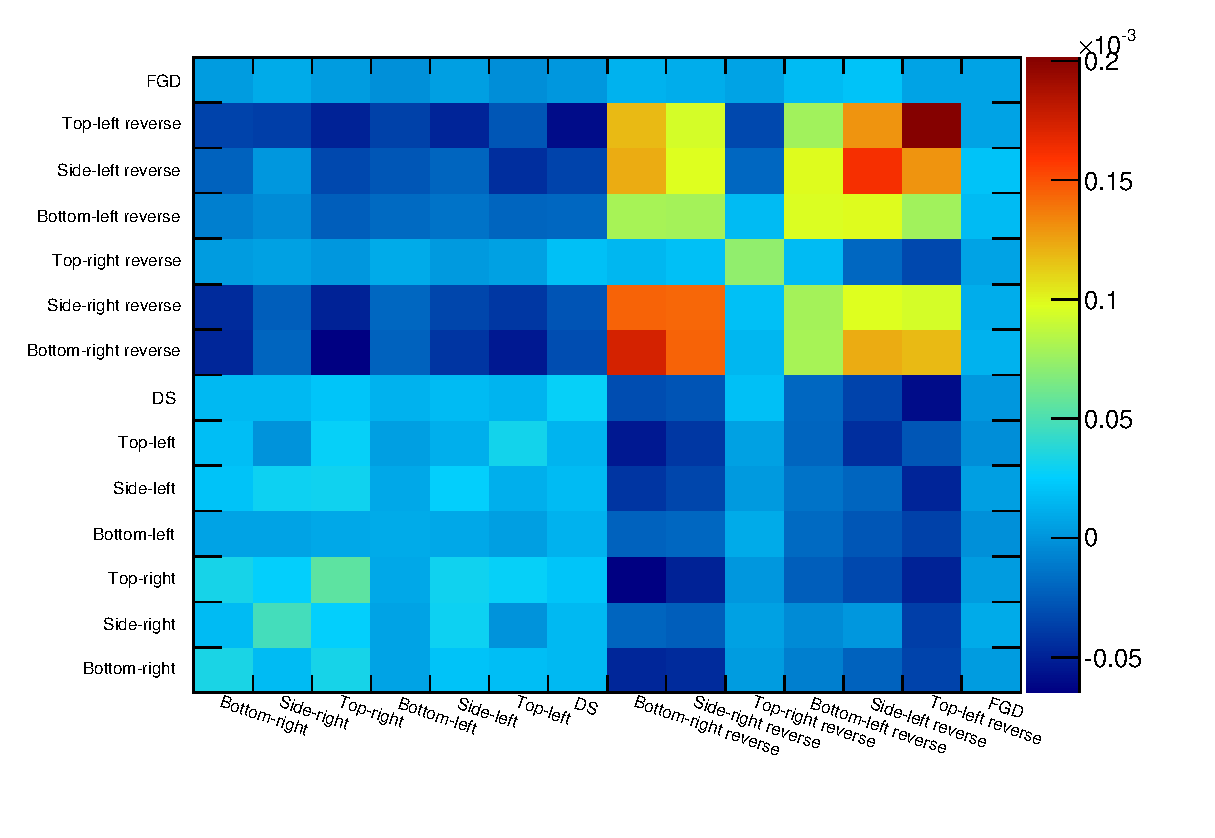
\includegraphics[width=8cm]{images/measurement/systematics/xsec/fsi_covariance_matrix.eps} \label{fig:FSIShapeNormCovarianceMatrix}}
  \subfloat[Shape-only.]{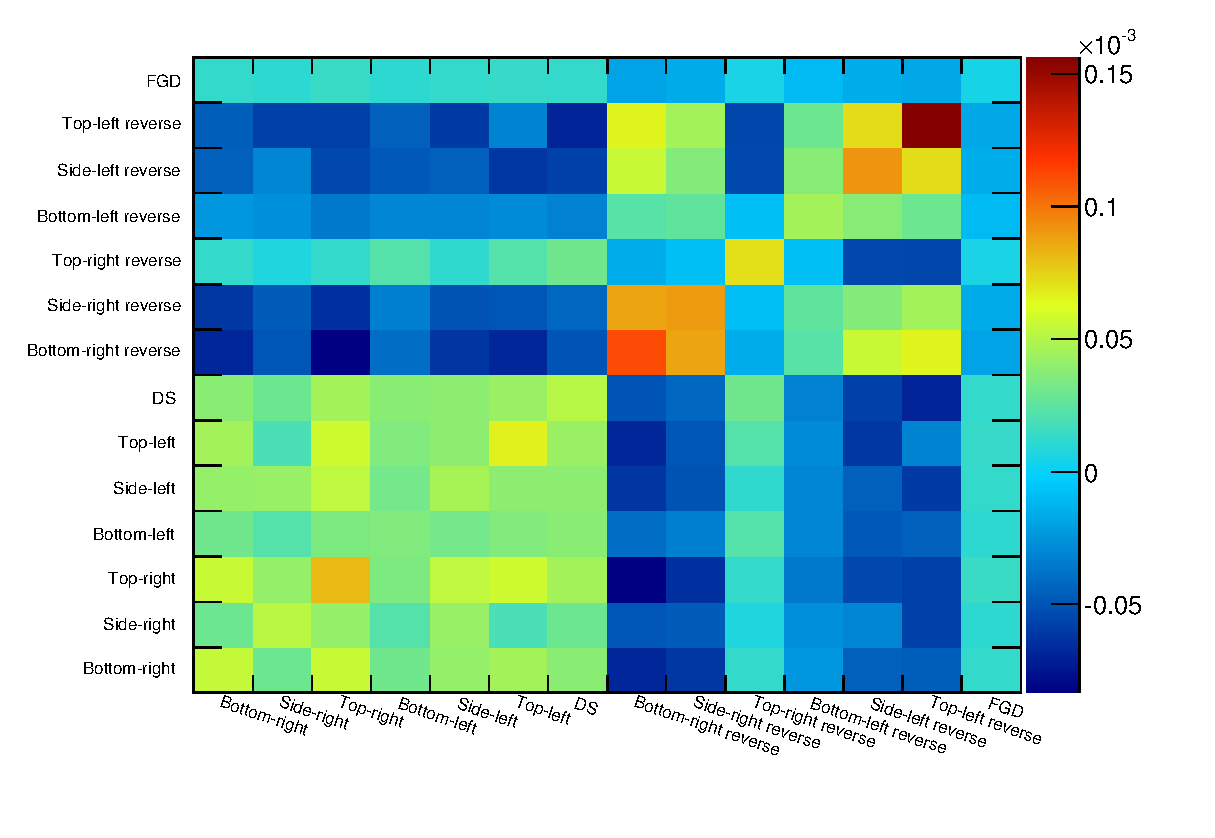
\includegraphics[width=8cm]{images/measurement/systematics/xsec/fsi_shape_covariance_matrix.eps} \label{fig:FSIShapeOnlyCovarianceMatrix}}
  \caption{The sample covariance induced by variation of of the FSI parameters outlined in table~\ref{table:FSIErrors}.}
  \label{fig:FSICovarianceMatrices}
\end{figure}
%really is just the number of in sample a for throw $i$ after applying the event weights.  For the shape-only covariance matrix, $N_{\textrm{a}}^{i}$ is defined as 
%\begin{equation}
%  N_{\textrm{a}}^{i} = 
%\end{equation}
\subsection{ECal detector systematic evaluation}
\label{subsec:ECalDetectorSystematic}
The analysis presented makes heavy use of a computational model of the ND280 ECal.  Any differences between this model and the real ND280 ECal could cause a systematic difference between the analysed Monte Carlo and the collected data used in this study.  So, several key areas have been identified which could cause such a systematic discrepancy, under the assumption that the differences exist.
\newline
\newline
The implemented selections uses the enhanced reconstruction, outlined in chapter~\ref{chap:EnhancedECalReconstruction}.  The enhanced reconstruction, depends on a set of clustering algorithms which are outlined in section~\ref{sec:ECalEventReconstruction} and the clustering algorithms depend on the hit scintillator bars themselves.  Following this trail back, it can be argued that the vast majority of the ECal detector systematics can be covered by assessing the ability of the ECal to reconstruct individual hits.  Specifically, the vast majority of the ECal's systematic uncertainty can be assessed by investigating the hit efficiency of the scintillator bars.  The aim of this study is to quantify the relative ECal hit inefficiency found from collected data and use that information to invoke a similar ECal hit inefficiency in the MC.  The effect of the hit inefficiency can then be propagated through the reconstruction and analysis to study its effect on the number of selected events.  Fig.~\ref{fig:LayerEfficiencyCosmicData} shows the layer-by-layer efficiency of the ND280 ECals, measured using cosmic data~\cite{1748-0221-8-10-P10019}.  Cosmic rays, which are largely composed of MIPs, are typically through going and only hit one bar per layer.  So, the efficiencies shown in Fig.~\ref{fig:LayerEfficiencyCosmicData}, can be used as a proxy for the hit efficiency of the scintillator bars.  Fig.~\ref{fig:LayerEfficiencyCosmicData} contains almost all of the necessary information required to study this systematic uncertainty with the only missing information being the hit efficiency of the MC ECal.  Due to time constraints, it was necessary to make a couple of conservative assumptions:
\begin{figure}
  \centering
  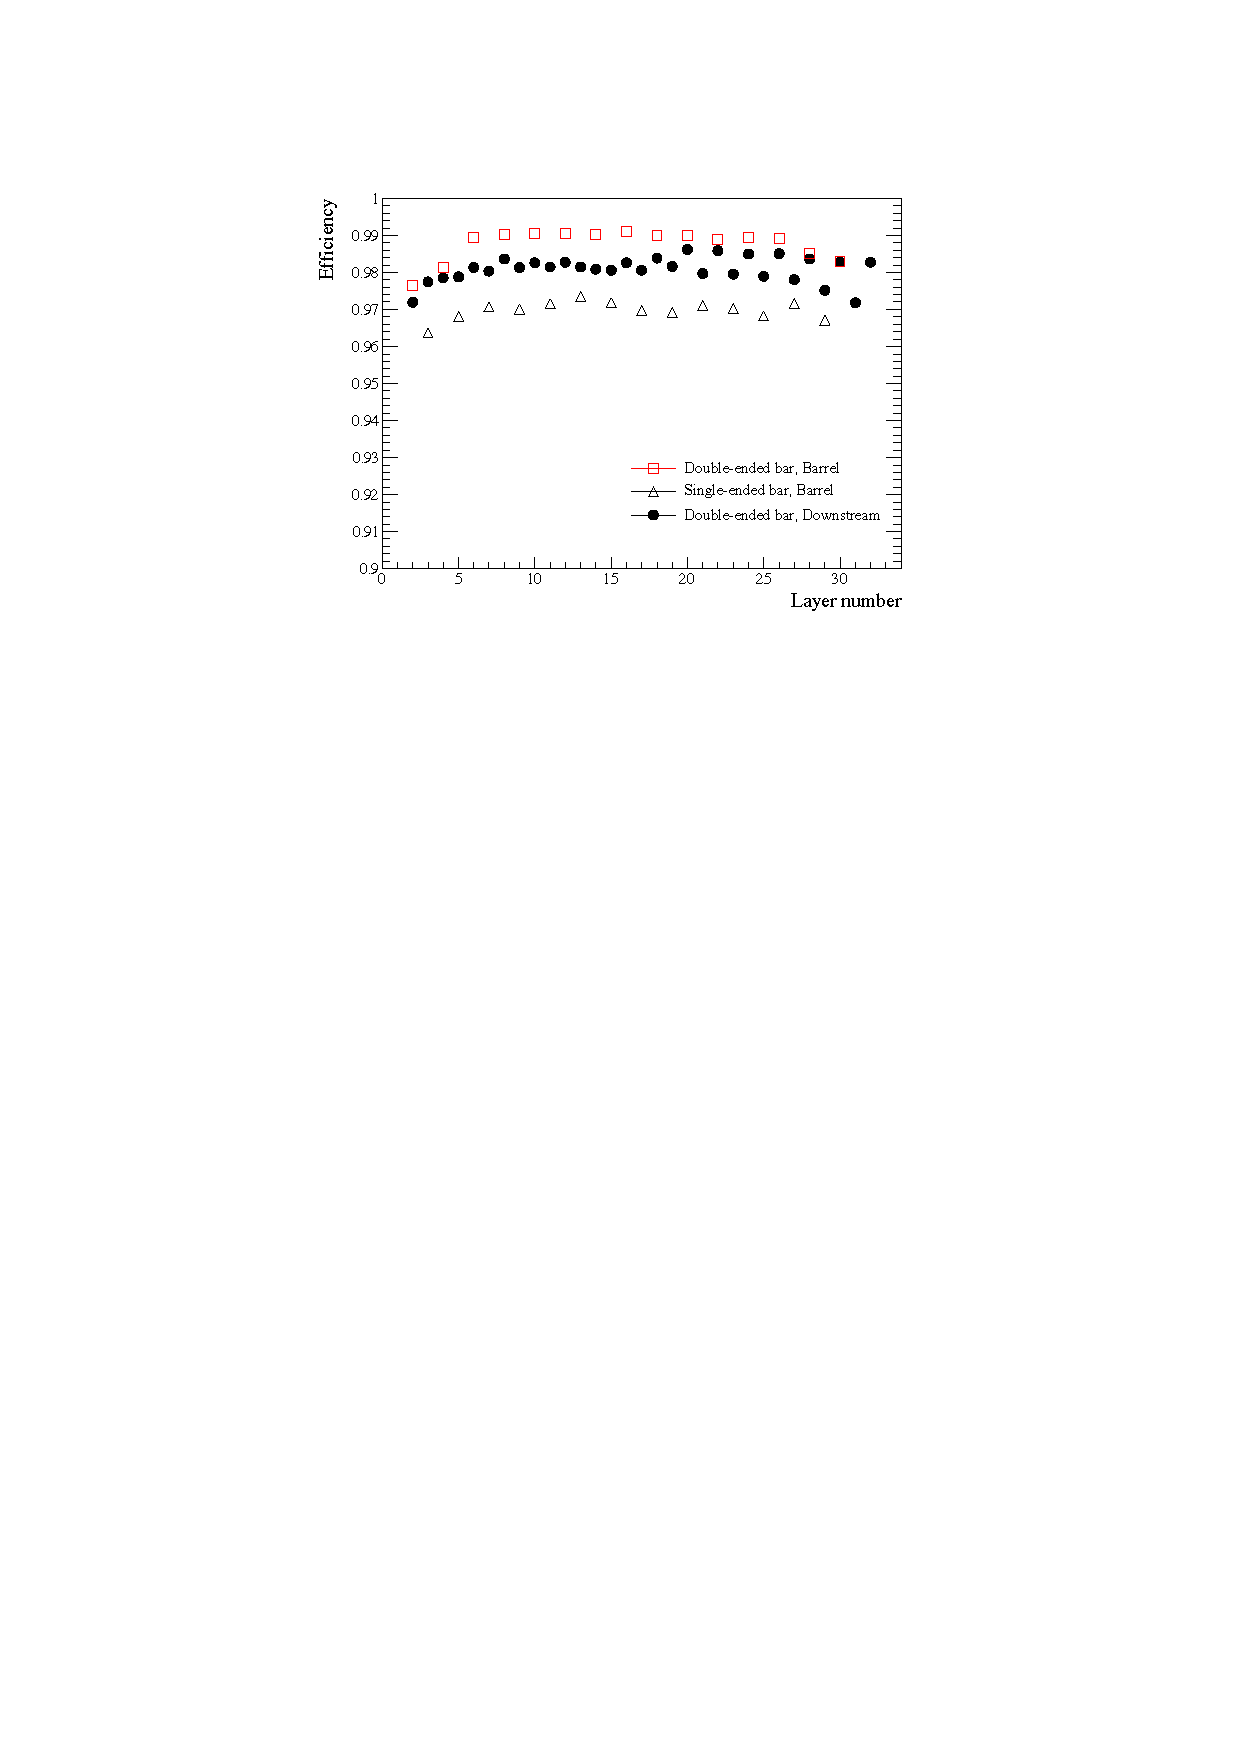
\includegraphics[width=10cm]{images/measurement/systematics/detector/threshold/layer_efficiency_cosmics_data.pdf}
  \caption{The layer-by-layer efficiency for the ND280 ECals, measured using cosmic data~\cite{1748-0221-8-10-P10019}.}
  \label{fig:LayerEfficiencyCosmicData}
\end{figure}
\begin{itemize}
\item The MC hit efficiency is 100$\%$.
\item The data hit efficiency for all bars is the lowest efficiency shown in Fig.~\ref{fig:LayerEfficiencyCosmicData}, which is 96.2$\%$.
\end{itemize}
Bearing the assumptions in mind, the hit inefficiency which must be applied to the MC is 3.8$\%$.  Care must be taken when attempting to apply the hit inefficiency to the MC.  Naivelly, one might attempt to randomly remove 3.8$\%$ of hits from the reconstruction, however this would not best represent the hit inefficiency.  There are many reasons why a scintillator bar would not be $100\%$ efficient, however the efficiency should correlate with the deposited charge.  So, to best model this systematic effect, the lowest 3.8$\%$ of hits should be removed from the MIP peak in charge space.  Fig.~\ref{fig:HitChargeCosmicMCPEU} shows the deposited charge for each hit created by MC cosmic rays.
\begin{figure}
  \centering
  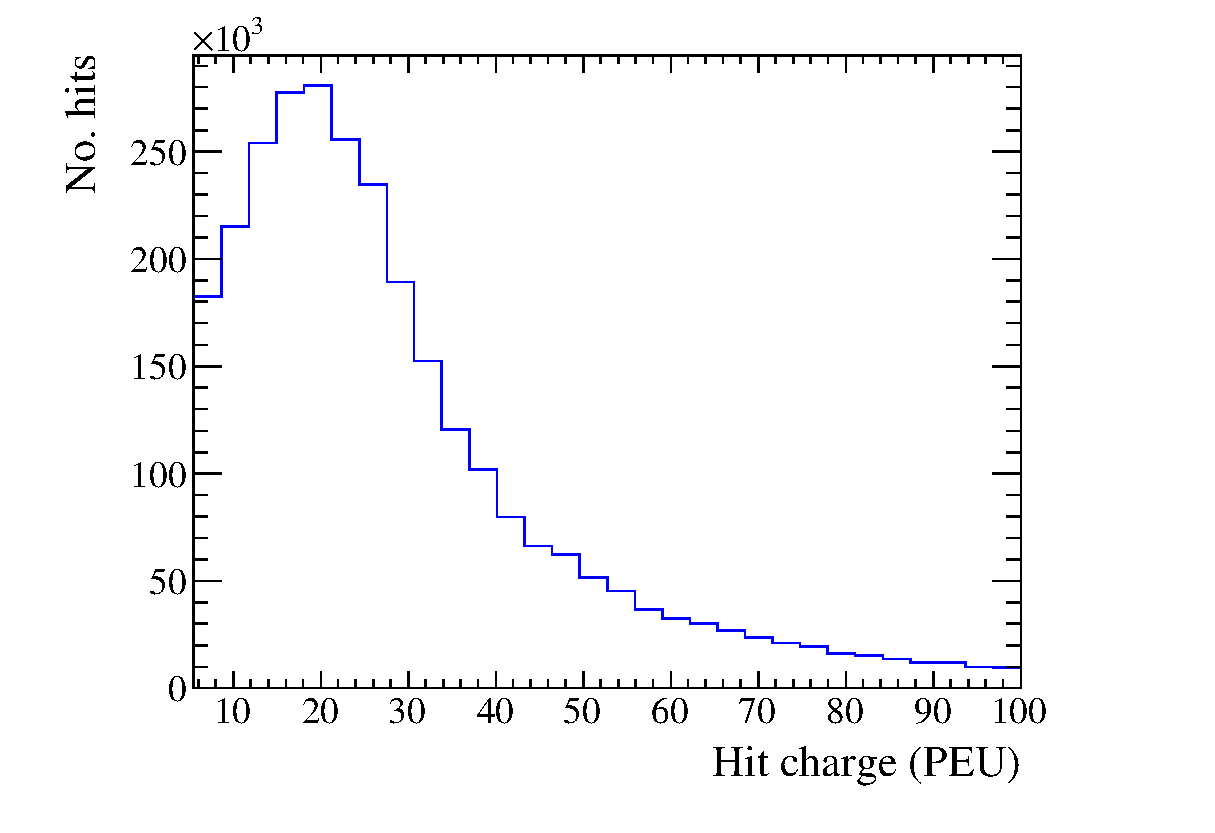
\includegraphics[width=10cm]{images/measurement/systematics/detector/threshold/hit_charge_cosmic_MC_PEU.eps}
  \caption{The charge distribution of scintillator bar hits created by MC cosmics rays.}
  \label{fig:HitChargeCosmicMCPEU}
\end{figure}
The distribution is cut off at 5.5 PEU, as this is a minimum threshold for output hits in the calibration stage of the ND280 software.  The clealy visible MIP peak is very close to this threshold and is actually partially cut off by this limit.  So, to apply the hit inefficiency, a new threshold needs to be calculated which removes an extra 3.8$\%$ of hits.  By calculating the lowest 3.8$\%$ of the hit charges created by the MC cosmic events, the new threshold hold was calculated to be 7.55 PEU.  This new threshold was applied as an initial stage of the reconstruction.  The recontruction and selection was then reapplied to the sample.  This new sample was then compared to the nominal sample to construct the covariance matrices, which are shown in Fig.~\ref{fig:ECalThresholdCovarianceMatrices}.  The largest uncertainty for the samples was found to be 3.74$\%$.
\begin{figure}%
  \centering
  \subfloat[Shape+normalisation.]{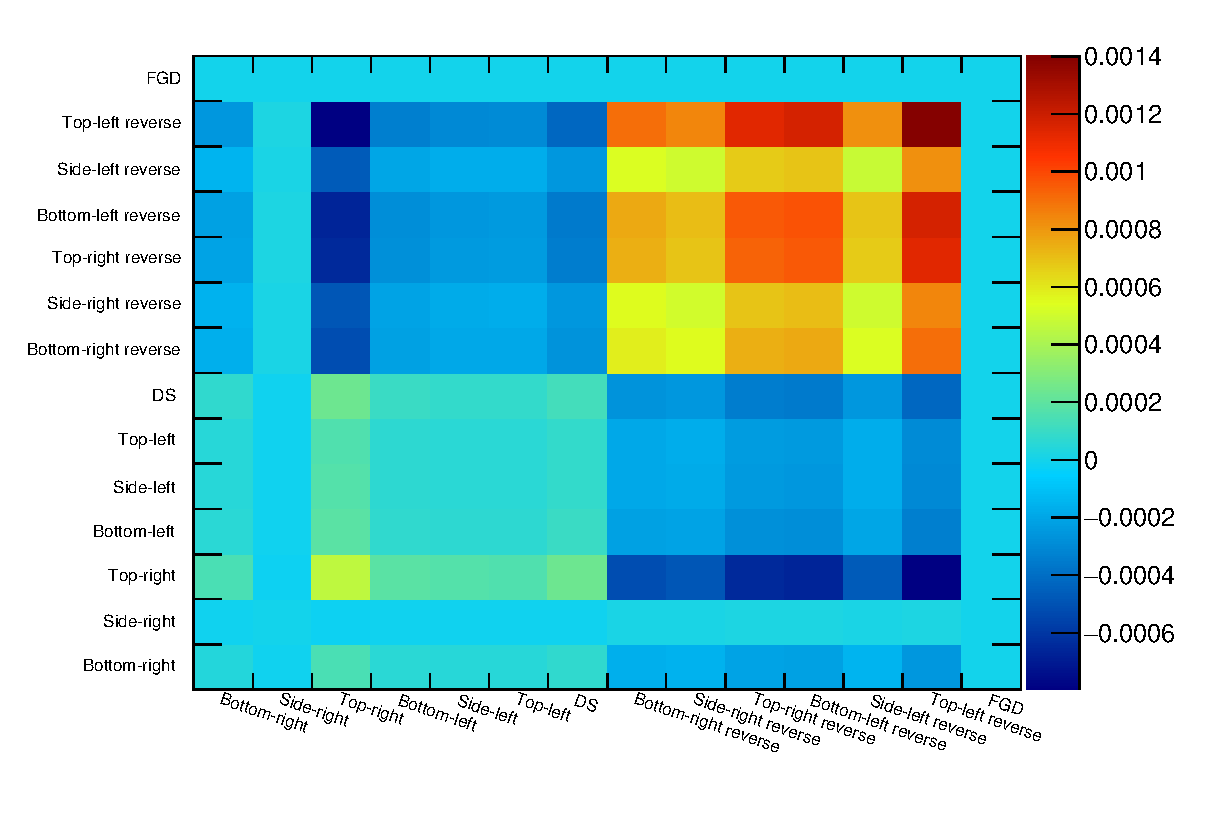
\includegraphics[width=8cm]{images/measurement/systematics/detector/threshold/ecal_threshold_covariance_matrix.eps} \label{fig:ECalThresholdShapeNormCovarianceMatrix}}
  \subfloat[Shape-only.]{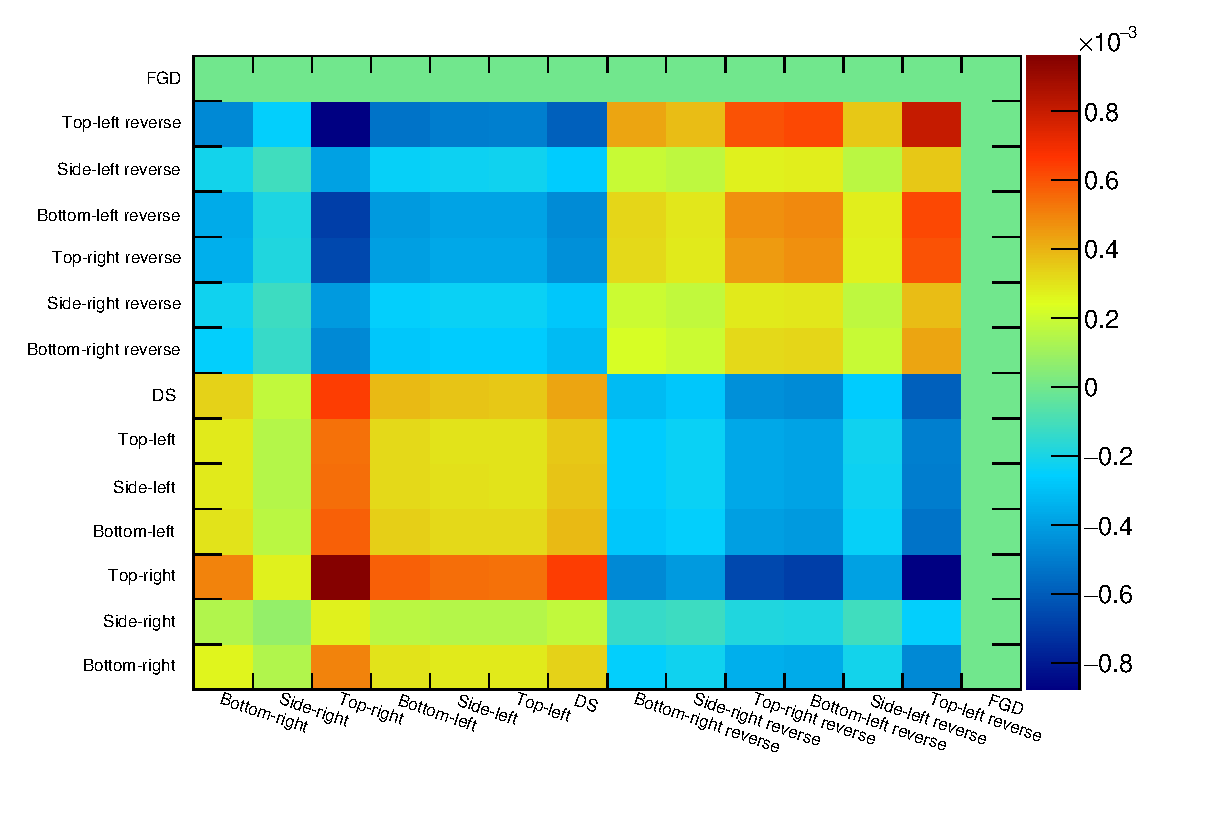
\includegraphics[width=8cm]{images/measurement/systematics/detector/threshold/ecal_threshold_shape_covariance_matrix.eps} \label{fig:ECalThresholdShapeOnlyCovarianceMatrix}}
  \caption{The sample covariance induced by the ECal hit inefficiency.}
  \label{fig:ECalThresholdCovarianceMatrices}
\end{figure}
\newline
\newline
The hit efficiency systematic uncertainty actually covers several areas of uncertainty.  Firstly, it addresses how a change in the core input to the reconstruction changes its output and so, by extension, addresses the efficiency of the reconstruction.  However, because the inefficiency is invoked by removing low charge hits, it also addresses how low charge hits, which could migrate below the minimum reconstruction threshold, could affect the analysis.  Because treatment of the charge by the hit efficiency systematic is partially covered, it is only necessary to additionally address how variation in the charge of the already reconstructed objects could alter the number of objects which pass the selection cuts.  To assess this, a well understood sideband sample is needed such that the hit charge in MC and data can be compared.  Any shift or smearing of the charge in data, relative to Monte Carlo must then be added to the reconstructed objects, which can then be passed through the selection, allowing the covariance matrix to be constructed.  To study the variation in the hit charge, a sample of cosmic MC and data was used.  The two samples were passed through the enhanced reconstruction and the charge of the hits associated to the reconstructed events were then analysed.  An example of the reconstructed hit charges is shown in Fig.~\ref{fig:HitChargeNominalCosmicsTLB}.  
\begin{figure}%
  \centering
  \subfloat[Data and nominal MC.]{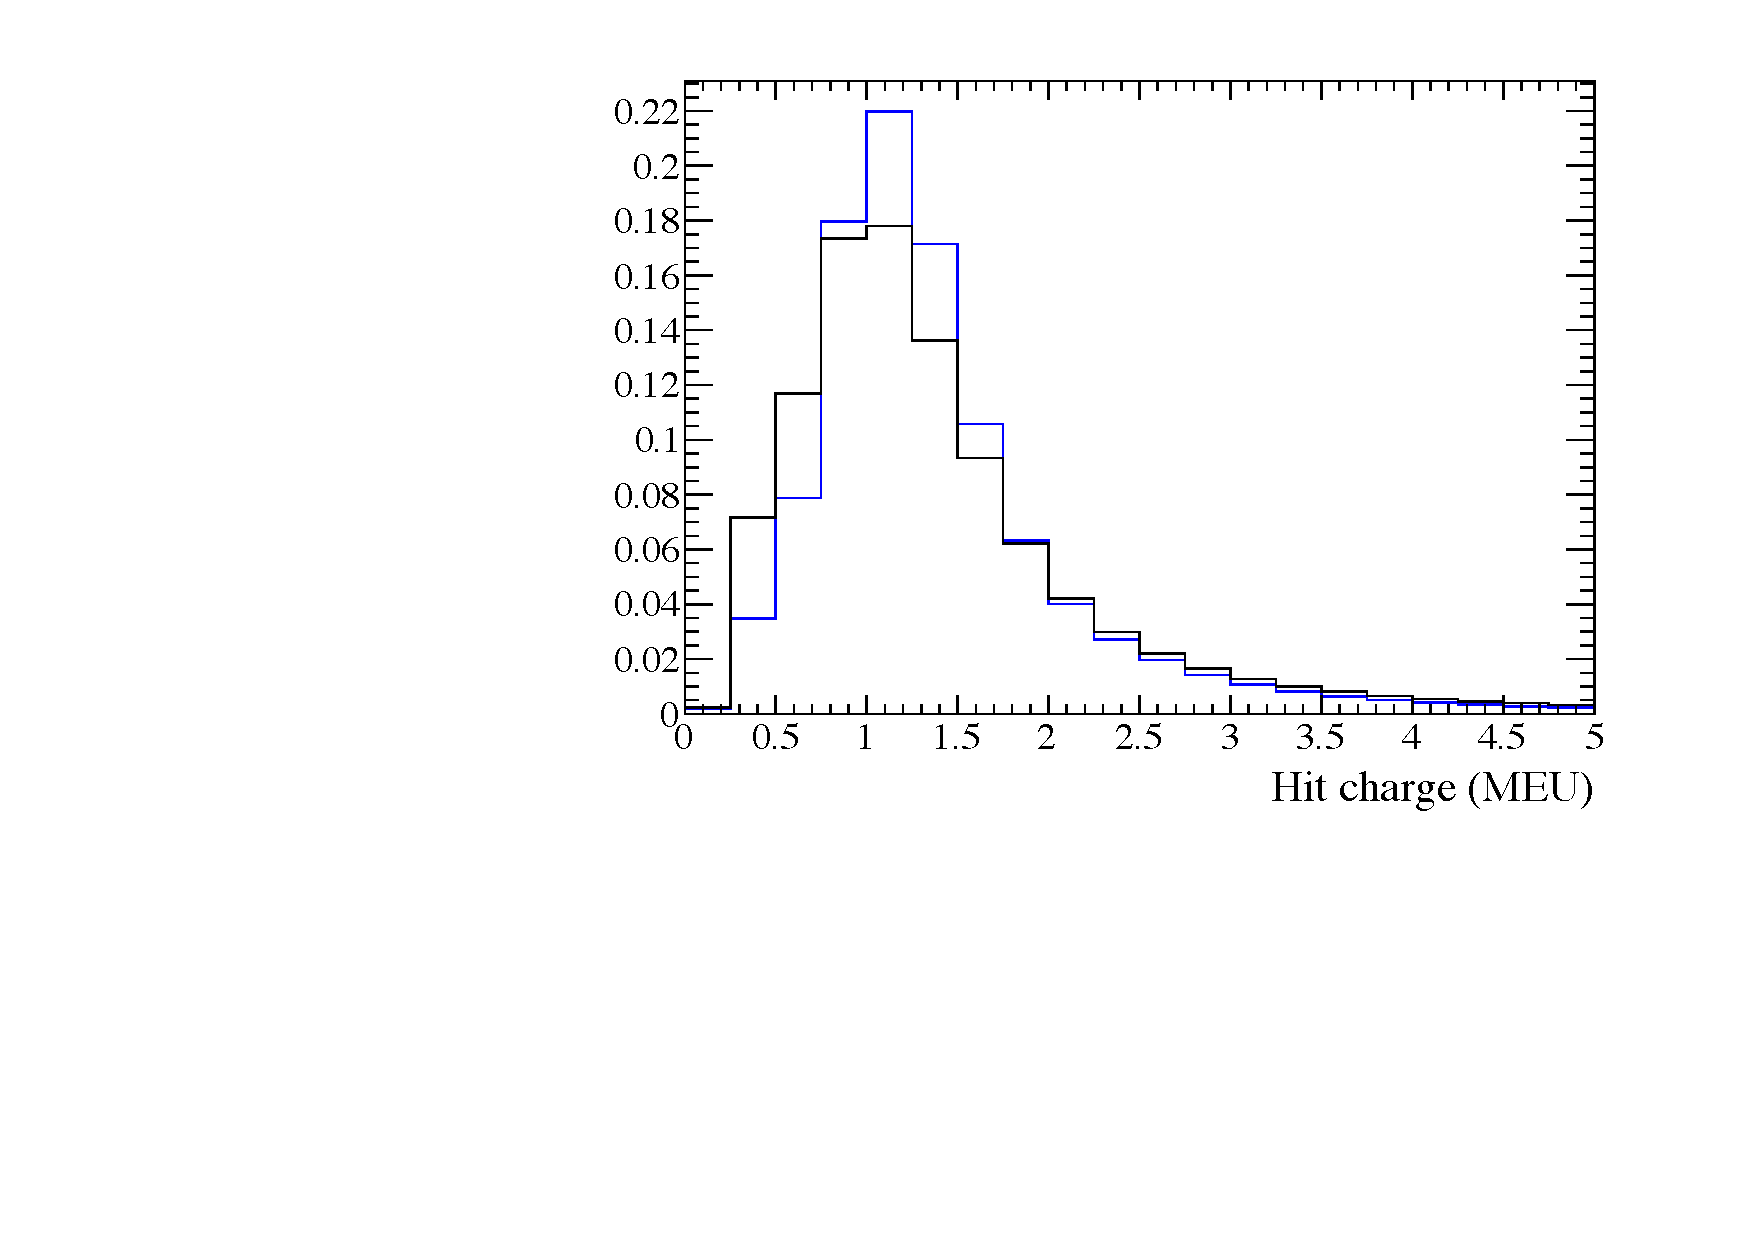
\includegraphics[width=8cm]{images/measurement/systematics/detector/charge/HitCharge_Cosmics_TLB.pdf} \label{fig:HitChargeNominalCosmicsTLB}}
  \subfloat[Data and shifted+smeared MC.]{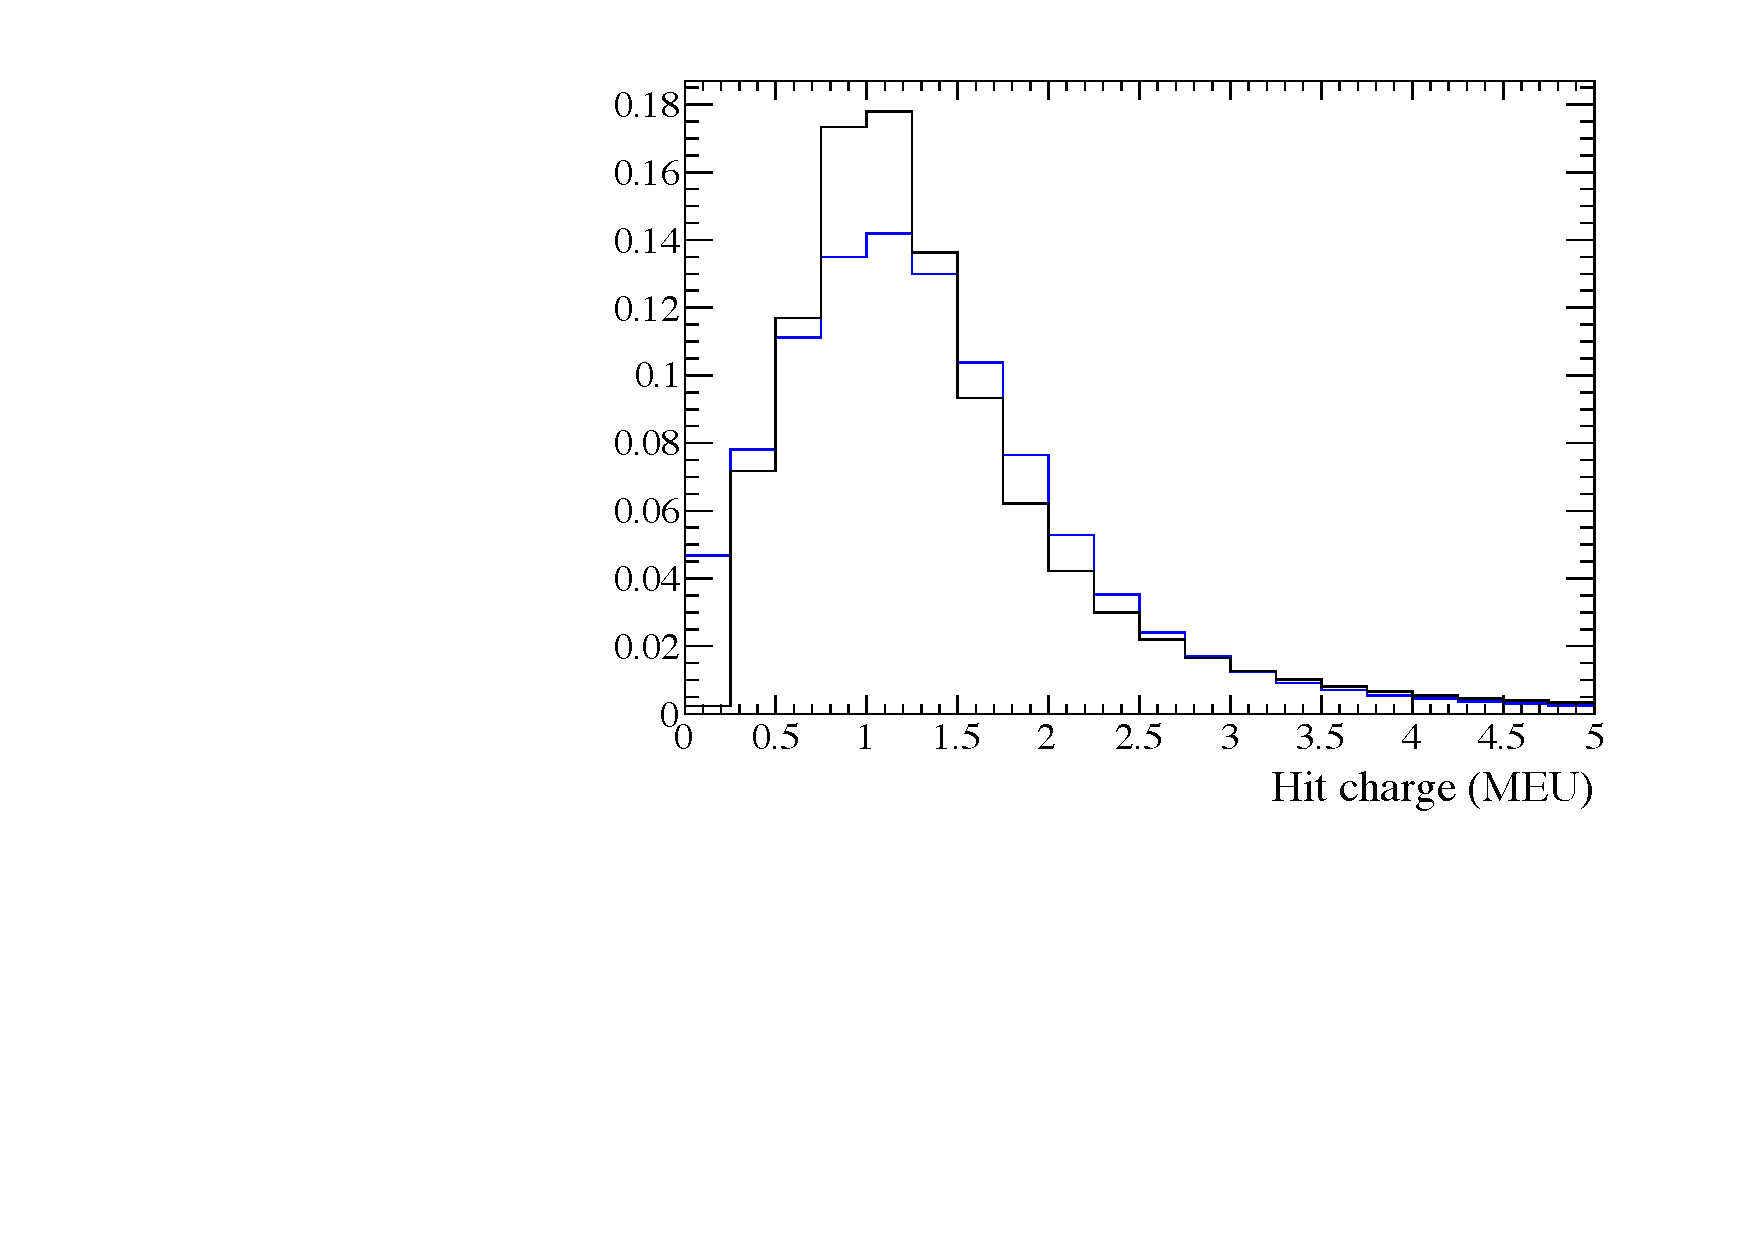
\includegraphics[width=8cm]{images/measurement/systematics/detector/charge/HitChargeCorrected_Cosmics_TLB.pdf} \label{fig:HitChargeCorrectedCosmicsTLB}}
  \caption{The charge of ECal hits after applying the enhanced reconstruction to run 3C cosmic events.  The distributions only show information for reconstructed objects in the top-left barrel ECal module.  The blue and black histograms are Monte Carlo and data respectively.}
  \label{fig:ECalThresholdCovarianceMatrices}
\end{figure}
There are clear differences in the shape of the two distributions; the data charge peak is wider than the MC peak.  To quantify this difference in the peak of the distributions, a gaussian was fit to the top 66$\%$ of the two peaks which were then compared.  The relevant parameters for the comparison are the width of the data and MC fits, $\sigma_{\textrm{Data}}^{Q}$ and $\sigma_{\textrm{MC}}^{Q}$ respectively, and 
\begin{equation}
\Delta^Q = \mu_{\textrm{Data}}^Q - \mu_{\textrm{MC}}^Q,
\end{equation}
where $\mu_{\textrm{Data}}^Q$ and $\mu_{\textrm{MC}}^Q$ are the mean of the data and MC fits respectively.  $\Delta^Q$ measures the shift of the MC peak relative to data, while $\sigma_{\textrm{Data}}^{Q}$ and $\sigma_{\textrm{MC}}^{Q}$ can be used to quantify the relative width.  These values are shown in table~\ref{table:HitChargeFitValues}.  To truly quantify the difference in the charge distributions, not only is a well understood sample required, but also a clean set of reconstructed events to remove any additional effects which may mask the charge difference.  As the cosmic events will generally be be almost parallel to the vertical axis, only the top and bottom ECal modules will be able to cleanly reconstruct the cosmics events, so only those events should be considered.  Ideally, the values shown in table~\ref{table:HitChargeFitValues}, would be used to correct and smear the MC peak to match data.  
\begin{table}
  \begin{tabular}{ c c c c }
   ECal module & $\Delta^{Q}$ (MEU) & $\sigma_{\textrm{Data}}^Q$ (MEU) & $\sigma_{\textrm{MC}}^Q$ (MEU) \\ \hline \hline
   Bottom-right & -0.095 & 0.37 & 0.51 \\
   Bottom-left & +0.045 & 0.37 & 0.61 \\
   Top-right & -0.003 & 0.38 & 0.58 \\
   Top-left & -0.099 & 0.38 & 0.50 \\ \hline
   Side-right & -0.225 & 0.83 & 0.64 \\
   Side-left & -0.315 & 0.85 & 0.55 \\
   DS & -0.472 & 0.87 & 0.46 \\
  \end{tabular}
  \caption{Summary of the lead aborbers for the ND280 tracker ECals~\cite{1748-0221-8-10-P10019}.}
  \label{table:HitChargeFitValues}
\end{table}
However, due to time constraints, it was only possible to use said values to over-correct and over-smear the MC.  In terms of the individual hits, this meant using $\Delta^{Q}$ and $\sigma_{\textrm{Data}}^Q$ for the top-left ECal to apply a correction and smearing to the hit charge, regardless of which module the hit occurred in.  This is because the top-left ECal module has the largest value of $\Delta^{Q}$.  The adjusted hit charge is
\begin{equation}
Q' = Q + X
\label{eqn:HitChargeCorrection}
\end{equation}
where $Q$ is the nominal hit charge and $X$ is a random variable which is defined as 
\begin{equation}
X \sim N(\Delta^{Q},\sigma_{\textrm{Data}}^Q).
\label{eqn:HitChargeRandomVariable}
\end{equation}
It is important to note here that the width of the Gaussian distribution in which the adjustment is drawn from is $\sigma_{\textrm{Data}}^Q$.  By using this width, the MC hit charge is over-smeared relative to data.  An example application of equation~\ref{eqn:HitChargeCorrection} is shown in Fig.~\ref{fig:HitChargeCorrectedCosmicsTLB} which uses the same hit information as that in Fig.~\ref{fig:HitChargeNominalCosmicsTLB}, but with the correction applied to the MC hit charge.  As can be seen by comparing the two figures, the application of the over-smearing has caused the MC charge peak to be wider than the data peak.  To propagate the effect of this systematic, this smearing and correction needs to be applied to the reconstructed prongs before any selection takes place.  Unfortunately, hit level information is not available at the level where the selection is applied.  So, a slightly modified charge adjustment is needed.  If the total charge contained on a prong is $Q_{\textrm{prong}}$, then the total adjusted charge is
\begin{equation}
Q'_{\textrm{prong}} = Q_{\textrm{prong}} + X_{\textrm{prong}}
\label{eqn:ProngChargeRandomVariable}
\end{equation}
where $X_{\textrm{prong}}$ is a random variable and is defined as
\begin{equation}
X \sim N(\Delta^{Q}N_{\textrm{prong}},\sigma_{\textrm{Data}}^Q),
\label{eqn:HitChargeRandomVariable}
\end{equation}
where $N_{\textrm{prong}}$ is the number of hits contained on the prong.  Following the above description, the prong charge variation was applied to every reconstructed prong in the systematic sample and the selection was then applied.  This process was repeated 1000 times to build up the covariance matrices, which are shown in Fig.~\ref{fig:ECalChargeCovarianceMatrices}.
\begin{figure}%
  \centering
  \subfloat[Shape+normalisation.]{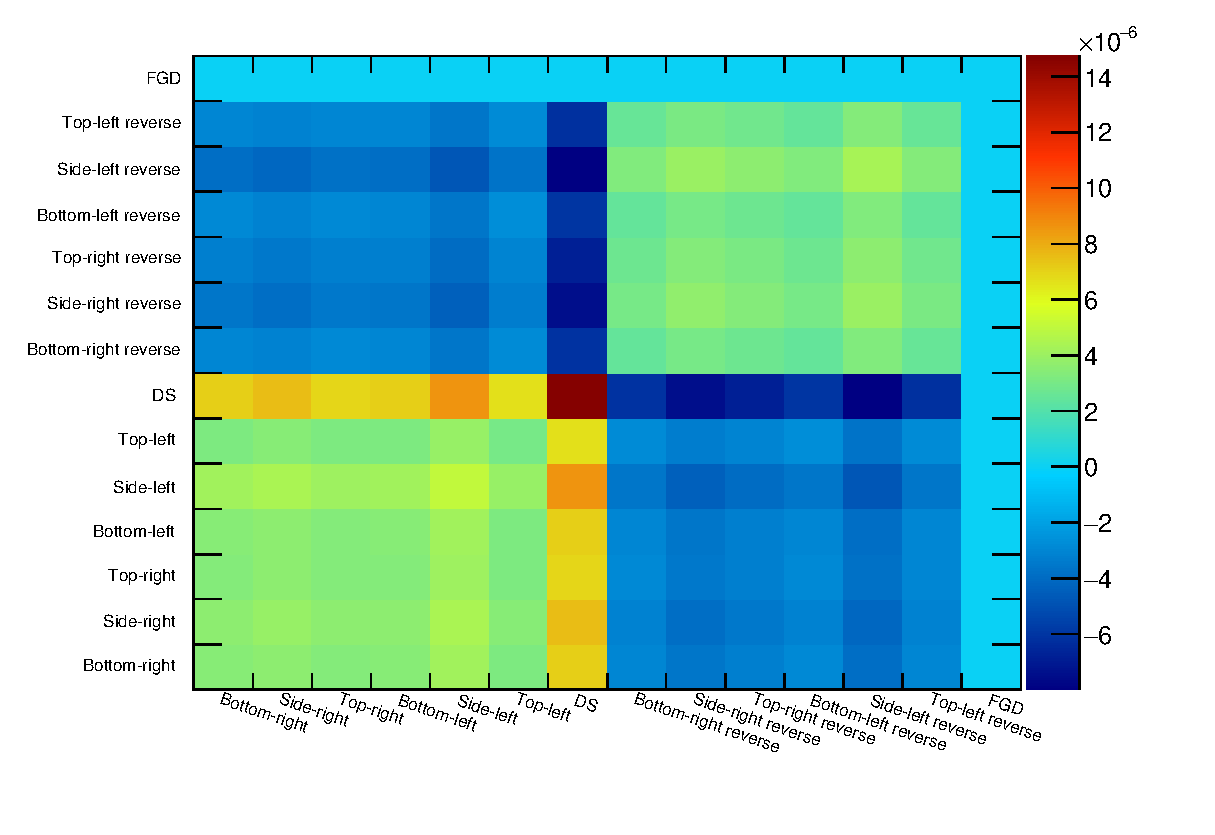
\includegraphics[width=8cm]{images/measurement/systematics/detector/charge/ecal_charge_covariance_matrix.eps} \label{fig:ECalChargeShapeNormCovarianceMatrix}}
  \subfloat[Shape-only.]{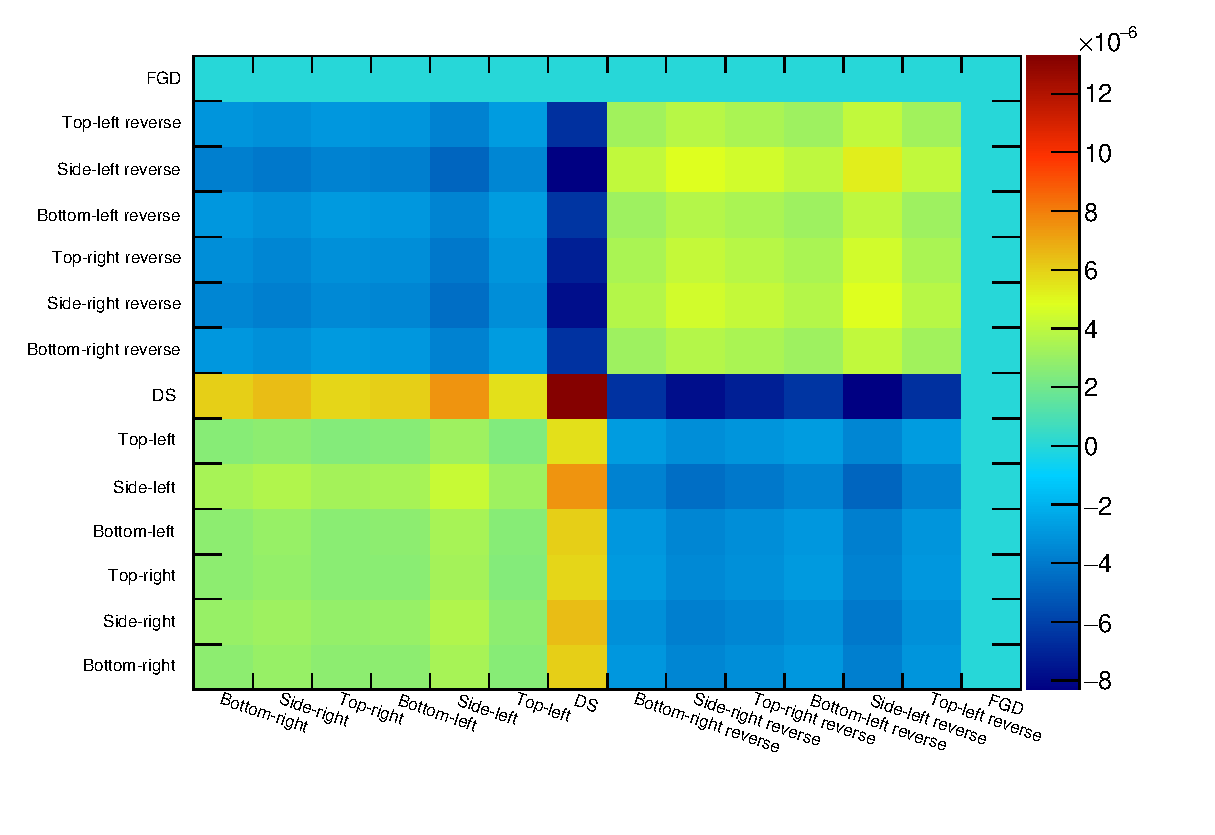
\includegraphics[width=8cm]{images/measurement/systematics/detector/charge/ecal_charge_shape_covariance_matrix.eps} \label{fig:ECalChargeShapeOnlyCovarianceMatrix}}
  \caption{The sample covariance induced by the ECal charge uncertainties.}
  \label{fig:ECalChargeCovarianceMatrices}
\end{figure}
\newline
\newline
The ECal model used in the simulation was based on the as built drawings and so should be an accurate model.  However, the components of each ECal module do have associated uncertainties which are not, and can not easily be, taken into account in the simulation, but could easily cause a systematic difference between data and Monte Carlo.  For example, if the DS ECal lead absorbers were thicker in the simulated model, one should expect to see a relative deficit of beam triggered events in the DS ECal collected data.  Provided that the component dimensions, compositions and uncertainties are known, toy Monte Carlo can be used to construct a set of toy ECal modules which model the variation in the module mass.  This can be expanded further, to construct a covariance matrix for the mass of each contributing element.  This covariance matrix can then be used to re-weight the events, based on target element, in the Monte Carlo sample to model the effect of the ECal mass systematic.  The ECal module designs are split into three types: side, top/bottom and DS.  It is only necessary to generate a mass covariance matrix for each of the three types.  All values used for the component dimensions/uncertainties are taken from [INSERT JINST REFERENCE].  Precise component dimensions are only quoted for the components in the active regions of each module, namely the lead absorbers, the scintillator bars and the wavelength-shifting fibres, so only these components are considered in the toy Monte Carlo study.  A summary of the components are shown in table~\ref{table:SideECalComponents}, table~\ref{table:TopBottomECalComponents} and table~\ref{table:DSECalComponents} for the side, top/bottom and DS ECal designs respectively.
\begin{table}
  \begin{tabular}{ c c c c }
     & Top/Bottom & Side & DS \\ \hline \hline
  No. per layer & 2 & 4 & 2 \\
  Length (mm) & $3858\pm4$ & $964.5\pm4$ & $2016\pm1$ \\
  Width (mm) & $765\pm4$ & $2330\pm4$ & $1008\pm4$ \\
  Height (mm) & $1.75\pm0.1$ & $1.75\pm0.1$ & $1.75\pm0.1$ \\
  Sb doping & $2.0\pm0.2\%$ & $2.0\pm0.2\%$ & $2.0\pm0.2\%$ \\
  \end{tabular}
  \caption{Summary of the lead aborbers for the ND280 tracker ECals~\cite{1748-0221-8-10-P10019}.}
  \label{table:LeadAbsorberDimensions}
\end{table}
\begin{table}
  \begin{tabular}{ c c c c }
     & Top/Bottom & Side & DS \\ \hline \hline
  No. per layer (para) & 38 & 57 & - \\
  No. per layer (perp) & 96 & 96 & 50 \\
  Length (para) (mm) & $3840\pm0.1$ & $3840\pm0.1$ & - \\
  Length (perp) (mm) & $1520\pm0.1$ & $2280\pm0.1$ & $2000\pm0.1$ \\
  Width (mm) & $40^{+0.0}_{-0.4}$ & $40^{+0.0}_{-0.4}$& $40^{+0.0}_{-0.4}$ \\
  Height (mm) & $10^{+0.0}_{-0.4}$ & $10^{+0.0}_{-0.4}$& $10^{+0.0}_{-0.4}$ \\
  Hole diameter (mm) & $1.75\pm0.1$ & $1.75\pm0.1$ & $1.75\pm0.1$ \\
  Composition (CH:PPO) & 99:1 & 99:1 & 99:1 \\
  Coating thickness (mm) & $0.25\pm0.13$ & $0.25\pm0.13$ & $0.25\pm0.13$ \\
  Coating composition (CH:TiO$_2$) & 85:15 & 85:15 & 85:15 \\

  \end{tabular}
  \caption{Summary of the scintillator bars for the ND280 tracker ECals~\cite{1748-0221-8-10-P10019}.}
  \label{table:ScintillatorBarDimensions}
\end{table}

\begin{table}
  \begin{tabular}{ c c c c }
     & Top/Bottom & Side & DS \\ \hline \hline
  No. per layer (para) & 38 & 57 & - \\
  No. per layer (perp) & 96 & 96 & 50 \\
  Length (para) (mm) & $3840\pm0.05$ & $3840\pm0.05$ & - \\
  Length (perp) (mm) & $1520\pm0.05$ & $2280\pm0.05$ & $2000\pm0.05$ \\
  Diameter (mm) & $1^{+0.02}_{-0.03}$ & $1^{+0.02}_{-0.03}$ & $1^{+0.02}_{-0.03}$\\
  Composition & CH & CH & CH \\

  \end{tabular}
  \caption{Summary of the WLSfibres for the ND280 tracker ECals~\cite{1748-0221-8-10-P10019}.}
  \label{table:WLSFibreDimensions}
\end{table}



%The following discusses the construction of the side toy ECal modules.  The choices made and the process followed were the same for all three designs.  
\subsubsection{The lead absorbers}
\label{subsubsec:ECalMassLeadAbsorbers}
Reference~\cite{1748-0221-8-10-P10019} provided a clear description of the composition of the lead absorbers for the ECal module designs, which are summarised in table~\ref{table:LeadAbsorberDimensions}.  All component uncertainties (both dimension and composition) were given as symmetric errors.  To construct an ECal lead layer, each layer dimension was systematically varied using a throw from a gaussian of mean 0 and a width of the dimension uncertainty.  After the layer volume was defined, the Sb contamination was calculated, also using a gaussian throw, but using a width of the Sb contamination uncertainty.  The described information could then be used to retrieve the mass of the Pb and Sb in anECal lead layer.

\subsubsection{The scintillator bars}
\label{subsubsec:ECalMassSctintillatorBars}
The information used to construct the toy scintillator bars is summarised in table~\ref{table:ScintillatorBarDimensions}, most of which was found in reference~\cite{1748-0221-8-10-P10019}.  The length of the bars were quoted with symmetric uncertainties (like the lead absorbers), so the length was also systematically varied using a throw from a gaussian of mean 0 and a width of the dimension uncertainty.  The hole and coating dimensions were also treated in the same manner.  However, the width and height were quoted with asymmetric errors and so could not be treated in the same way.  Fortunately, only a negative uncertainty was quoted, which meant the width and height uncertainties could be treated in a somewhat similar manner, but with randoms numbers being drawn from a half-gaussian.  The bar composition was reported as polystyrene doped with $1\%$~PPO (C$_{15}$H$_{11}$NO) and $0.03\%$~POPOP.  For the toy bar construction, the POPOP was considered negligable and so was not included.  The result is that the toy bar composition (excluding the coating) is 99$\%$~CH and 1$\%$~C$_{15}$H$_{11}$NO by mass.  Unfortunately, the full composition of the TiO$_2$ coating was extensively described.  However, a similar systematic study has already been undertaken for the FGD [FGD TN NOTE REFERENCE HERE] which included an investigation of the coating composition.  A representative for the Fermilab facility which extruded the scintillator bars reported that the final composition of the coating was 15$\%$ rutile-form TiO$_2$ and 85$\%$ CH with other contributing compounds considered negligable.  The collected information could then be used to retrieve the contributing mass of each element in a scintillator bar.

\subsubsection{The WLS fibres}
\label{subsubsec:ECalMassWLSFibres}
As with the other toy components, reference~\cite{1748-0221-8-10-P10019} provided most of the necessary information for the construction and could be largely treated in the same way.  The major difference is that the WLS fibre diameter had an asymmetric error in which both components were not zero.  So, two toy gaussians were constructed to draw from (one representing each uncertainty) and a random number was first drawn from a uniform distribution to decide which gaussian would be used.  Very little information was provided about the composition of the WLS fibre, however the mass study in the FGD [REFERENCE SCOTT OSER TECHNOTE] assumed the WLS fibre was composed entirely of scintillator, so the same assumption was used for this study.  As with the other components, the provided information could then be used to retrieve the contributing mass of the elements in the WLS fibres.

\subsubsection{ECal mass covariance}
\label{subsubsec:ECalMassCovariance}
Toy simulation was used to construct each component described in the above sections.  Each component was repeatedely built and was subsequently used to construct an ECal module.  The constributing mass of each element to the toy ECal module was then recorded.  10,000 toy ECal modules were constructed for each type, totalling 30,000 constructed modules.  The recorded contributing elemental mass for each construction was used to build up a mass covariance matrix using eqn.~\ref{eqn:CovarianceMatrixElementDef} and eqn.~\ref{eqn:NVariedDef}, an example of which is shown in Fig.~\ref{fig:MassCovDSECalAllElements} for the DS ECal.  Unfortunately, it was found that the covariance matrices for all three module types were singular, which is of immediate concern as the matrices need to be Cholesky decomposed as part of the systematic uncertainty evaluation.  It was found that the singular nature of the convariance matrices was caused by the contributing elements which have small covariance values (both on and off diagonal) and the problem could be solved by not considering some of them in the covariance matrix.  The three problematic elements are carbon, nitrogen and hydrogen.  Both nitrogen and hydgrogen only constitute a relatively small amount of the mass.  An example of this is shown in Fig.~\ref{fig:TotalMassDSECal} which shows the mass of the 10,000 toy DS ECal modules, with and without nitrogen and hydrogen.  There is a 2.45$\%$ difference between the two constructions which is borderline negligable.  While, ideally, the hydrogen and nitrogen should be included in the systematic evaluation, due to time constraints, they were excluded.  With the extra elements excluded, a non-singular covariance matrix for each module type could be constructed, all of which are shown in Fig.~\ref{fig:MassCovECalReducedElements}.
\begin{figure}
  \centering
  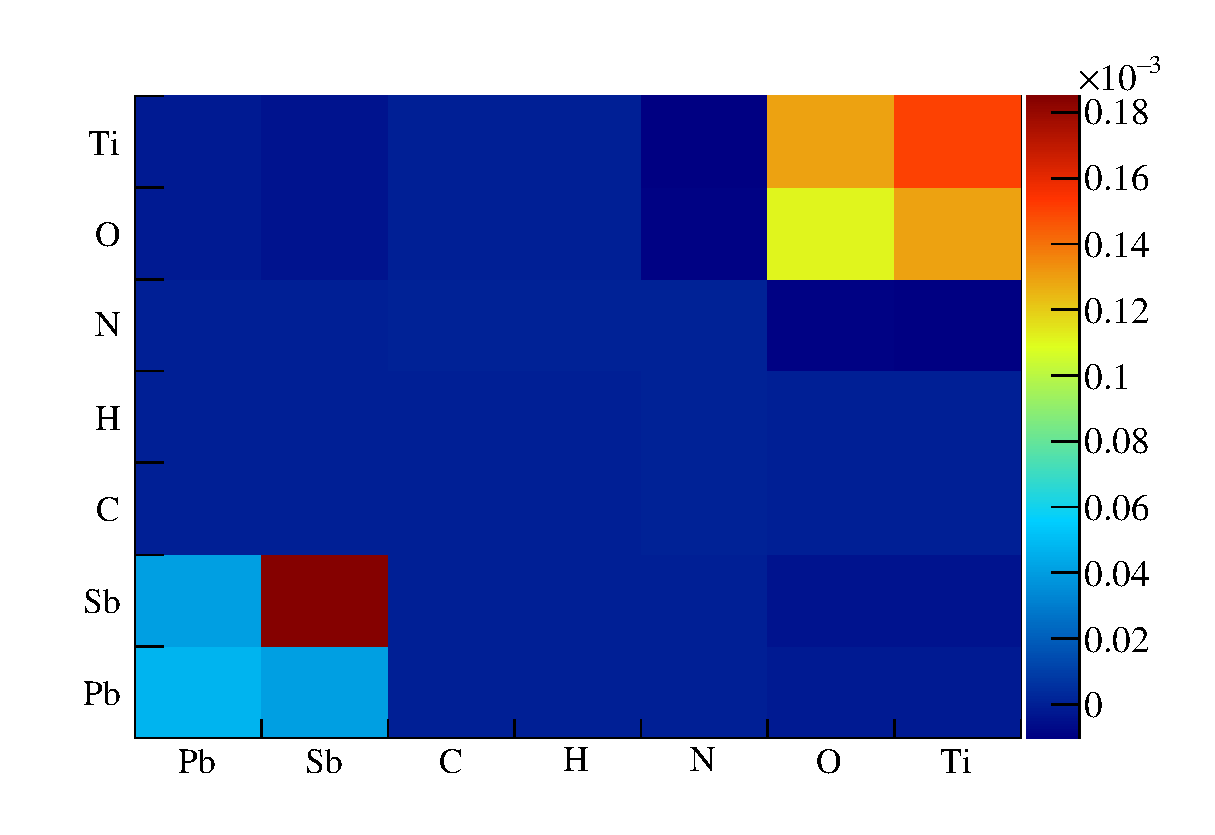
\includegraphics[width=10cm]{images/measurement/systematics/detector/mass/MassCov_DSECal_AllElements.eps}
  \caption{The covariance matrix for the mass of the contributing elements in the DS ECal, with all contributing elements considered.}
  \label{fig:MassCovDSECalAllElements}
\end{figure}
\begin{figure}
  \centering
  \includegraphics[width=10cm]{images/measurement/systematics/detector/mass/TotalMass_DSECal.eps}
  \caption{The total mass of the DS ECal active volume with (black) and without (blue) nitrogen and hydrogen as contributing elements.  The smooth lines are the Gaussian fits to the distributions.  Using the Gaussian mean and width as the mass central value and uncertainty respectively, the DS ECal active mass with (without) hydrogen and nitrogen is $4060\pm20$~kg ($3960\pm20$~kg).}
  \label{fig:TotalMassDSECal}
\end{figure}
\begin{figure}
\begin{minipage}{.5\linewidth}
  \centering
  \subfloat[Top/bottom ECal.]{\label{fig:MassCovTopBottomECalReducedElements}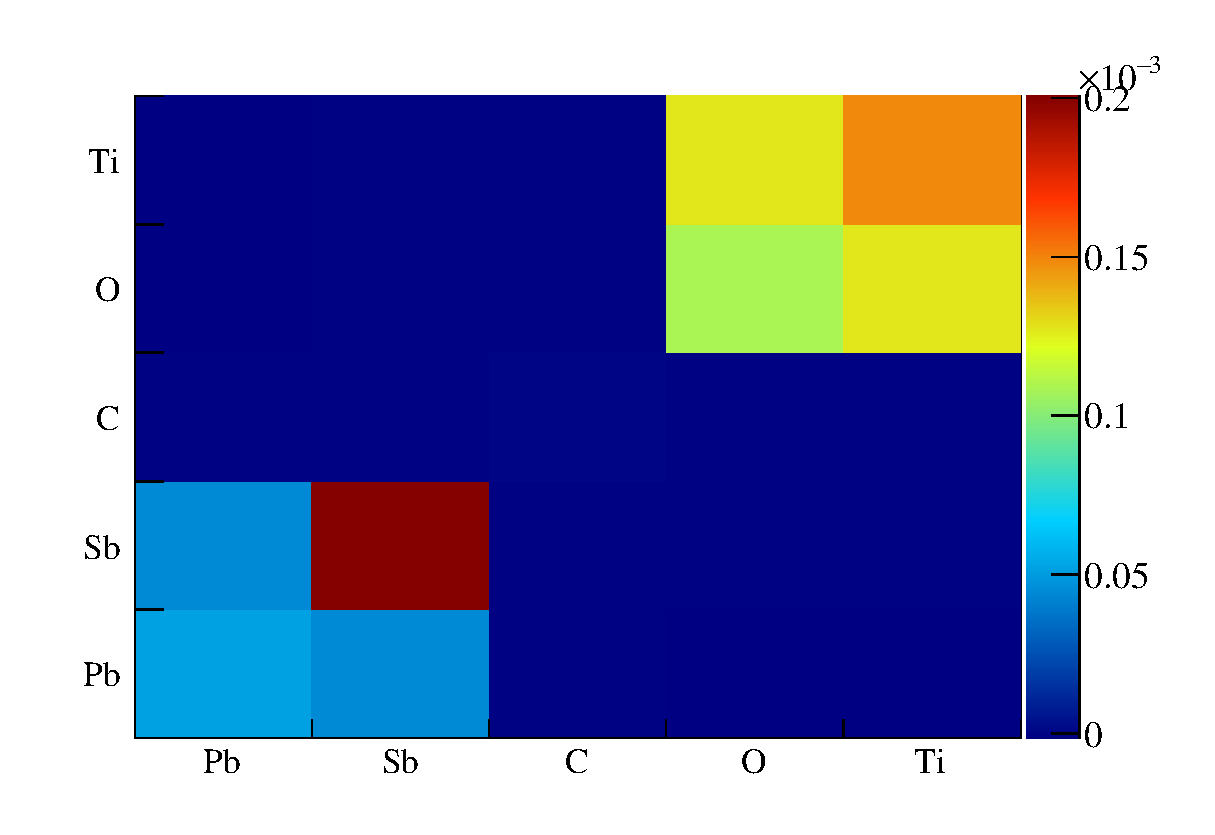
\includegraphics[width=7.5cm]{images/measurement/systematics/detector/mass/MassCov_TopBottomECal_ReducedElements.eps}}
\end{minipage}%
\begin{minipage}{.5\linewidth}
\centering
 \subfloat[Side ECal.]{\label{fig:MassCovSideECalReducedElements}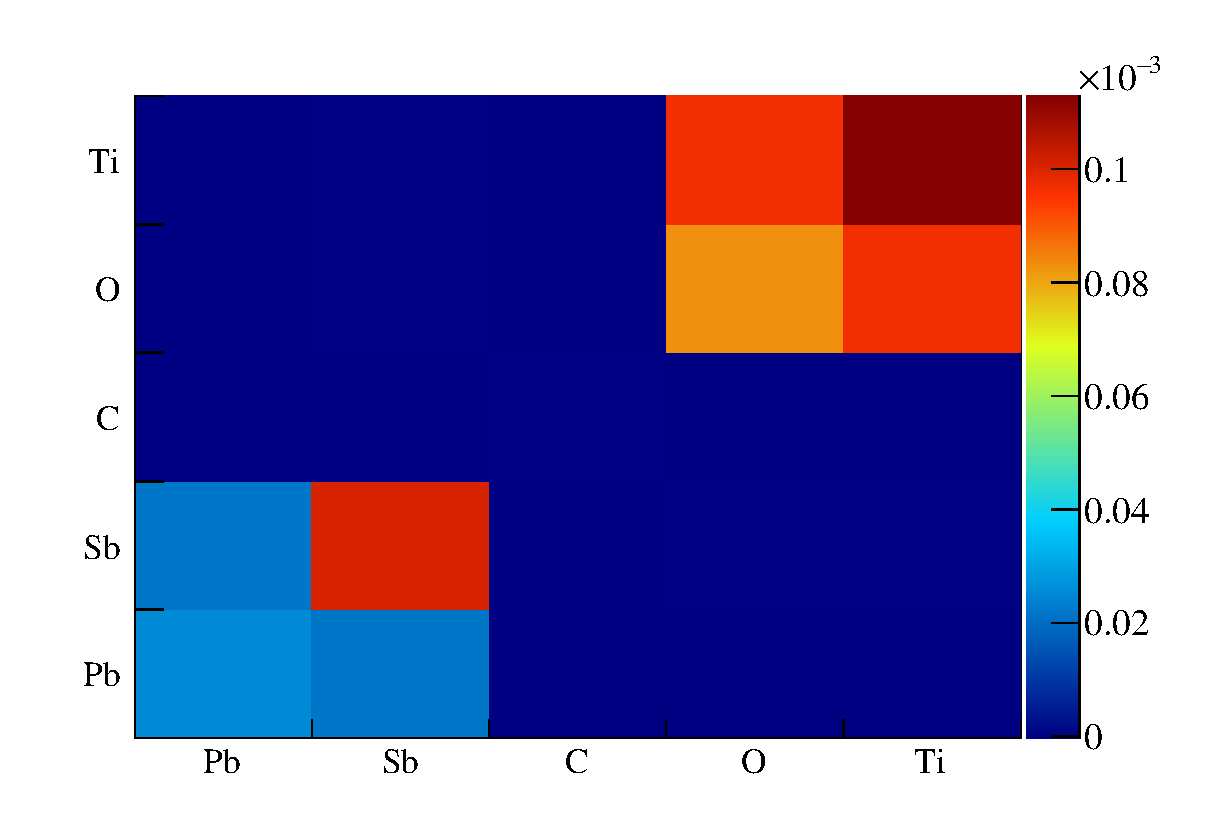
\includegraphics[width=7.5cm]{images/measurement/systematics/detector/mass/MassCov_SideECal_ReducedElements.eps}}

\end{minipage}\par\medskip
\centering
 \subfloat[DS ECal.]{\label{fig:MassCovDSECalReducedElements}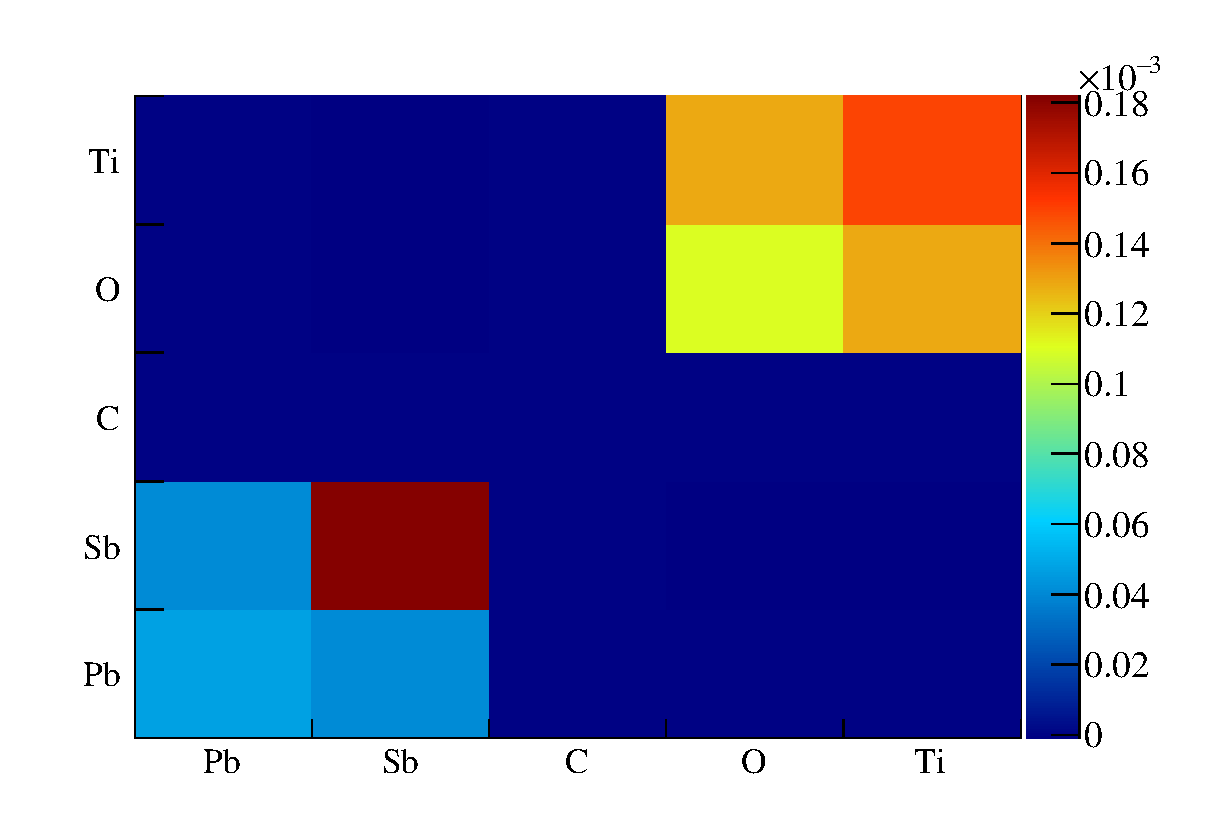
\includegraphics[width=7.5cm]{images/measurement/systematics/detector/mass/MassCov_DSECal_ReducedElements.eps}}

\caption{The fractional covariance matrix for the mass of each contributing element to an ECal module (hydrogen and nitrogen omitted).}
\label{fig:MassCovECalReducedElements}
\end{figure}
\subsubsection{Propagation of the mass systematic uncertainty}
\label{subsubsec:ECalMassSystematicPropagation}
The covariance matrices shown in Fig.~\ref{fig:MassCovECalReducedElements} were then used to generate systematic throws, in the same manner as the flux systematic uncertainty evaluation.  For the input into each systematic throw i.e. one run through of the selected Monte Carlo events, a set of event weights were generated for each of the seven ECal modules using the above mass covariance matrices.  Every neutrino interaction in the ECal active volume was weighted according to its target element.  As with the other systematic uncertainty evaluations, 1,000 systematic throws were generated and the subsequent covariance matrices were constructed which are shown in Fig.~\ref{fig:ECalMassCovarianceMatrices}.  The maximum uncertainty, which was for the DS ECal events, was found to be $0.39\%$. 
\begin{figure}%
  \centering
  \subfloat[Shape+normalisation.]{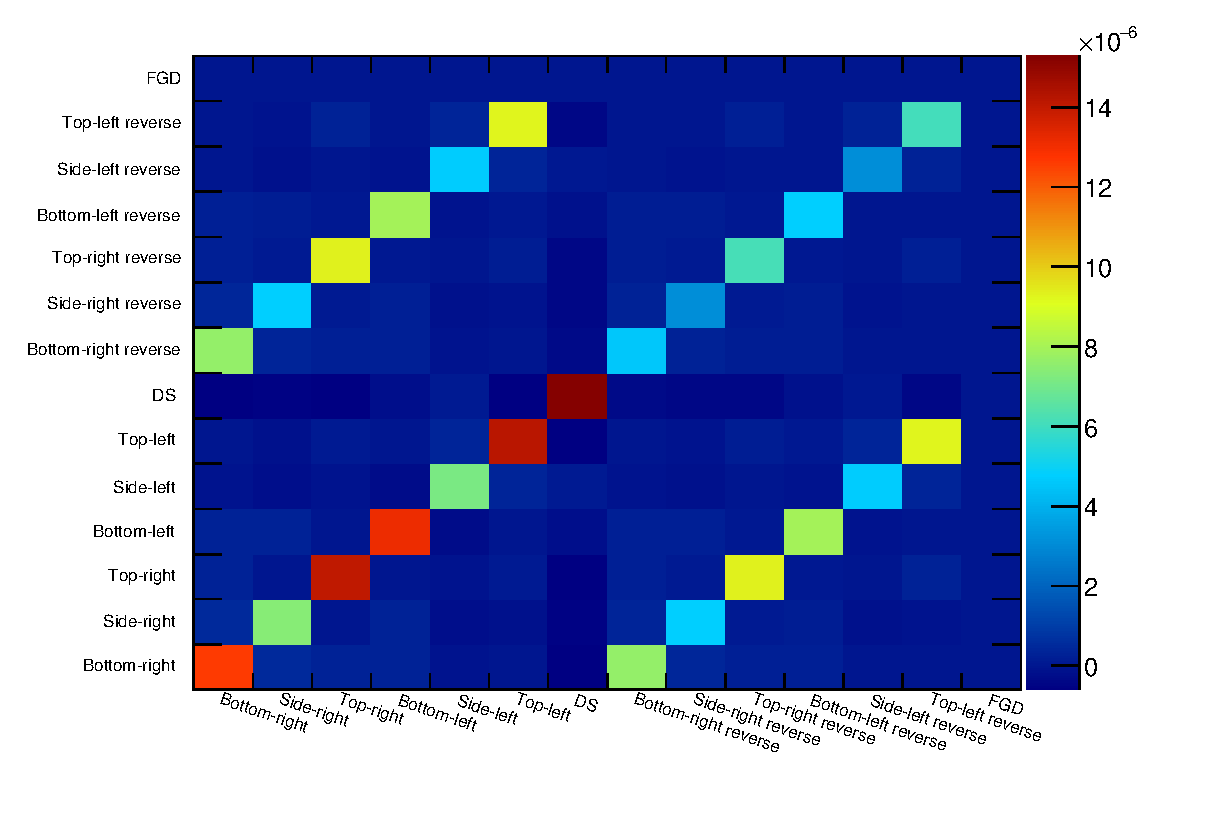
\includegraphics[width=8cm]{images/measurement/systematics/detector/mass/ecal_mass_covariance_matrix.eps} \label{fig:ECalMassShapeNormCovarianceMatrix}}
  \subfloat[Shape-only.]{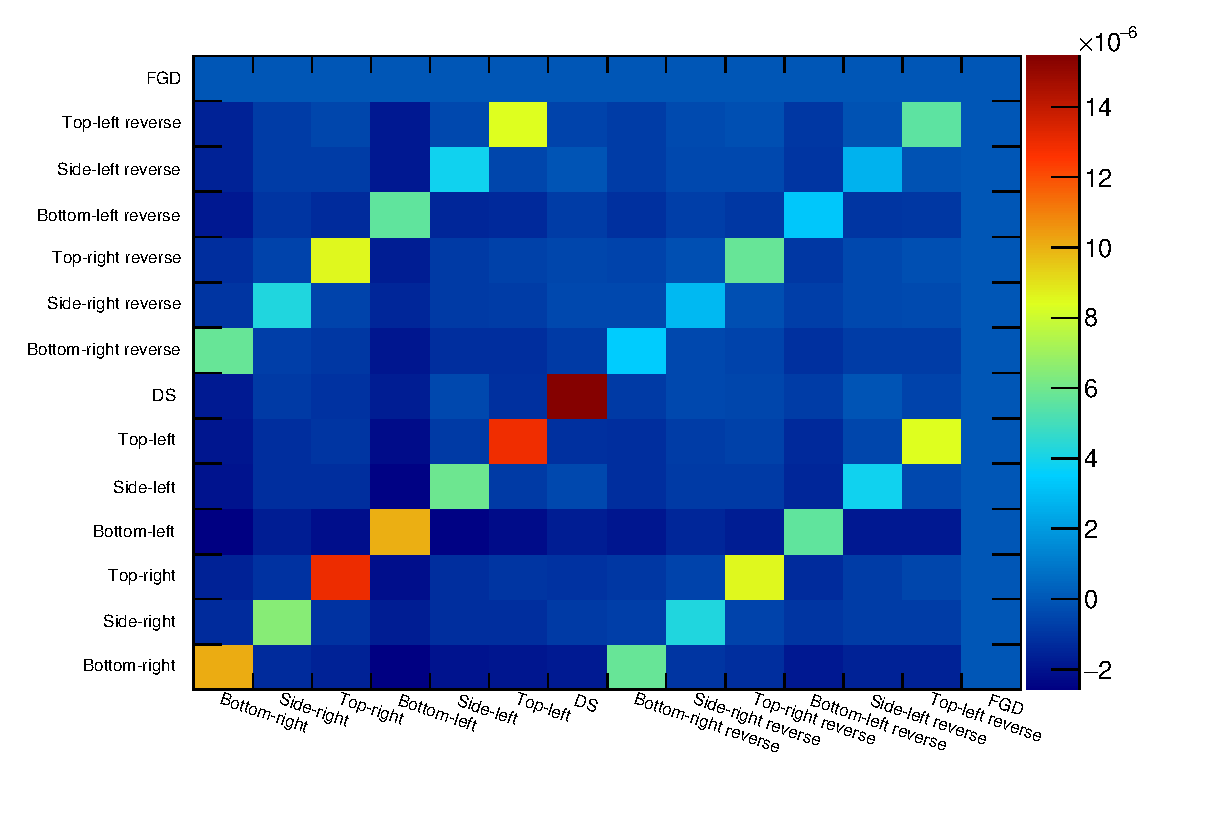
\includegraphics[width=8cm]{images/measurement/systematics/detector/mass/ecal_mass_shape_covariance_matrix.eps} \label{fig:ECalMassShapeOnlyCovarianceMatrix}}
  \caption{The sample covariance induced by the ECal mass uncertainties.}
  \label{fig:ECalMassCovarianceMatrices}
\end{figure}
\newline
\newline
An additional source of systeamtic uncertainty could come from the ECal's ability to reject OOFV backgrounds. As fig.~\ref{fig:ProngStackSelected} shows, the dominant background selected, particularly for the barrel ECals, is the OOFV background.  If the simulation of the ECal had a different OOFV background rejection capability to that of the actual ECal, the selected event composition between data and MC simulation would differ, resulting in a systematic difference.  The only feasable way to assess this systematic uncertainty is to use control samples.  Unfortunately, only $\mu$ based control samples were available during the analysis.  However, fig,~\ref{fig:ProngStackSelected} shows that the one prong topology, which contains the largest number of selected events, has the biggest OOFV background contamination and as Fig.~\ref{fig:SelOOFVEventSurvivalBarrel} and Fig.~\ref{fig:SelOOFVEventSurvivalDS} show, $\mu$s are the dominant particle species in the surviving OOFV background.  To assess the systematic uncertainty, the $\mu$ based control samples, both data and MC, are passed through the selection and the number of reconstructed events which pass the fiducial volume cut are recorded, $N_{\textrm{CS}}^{\textrm{pass}}$.  The efficiency of the fiducial volume cut is then defined as
\begin{equation}
\epsilon_{\textrm{CS}} = \frac{N_{\textrm{CS}}^{\textrm{pass}}}{N_{\textrm{CS}}},
\label{eqn:OOFVCSEfficiency}
\end{equation}
where $N_{\textrm{CS}}$ is the number of reconstructed control sample events which enter the selection.  It is important to note why $N_{\textrm{CS}}^{\textrm{pass}}$ counts the number of events which pass the fiducial volume cut, rather than as the number of events which pass all of the selection cuts.  The reason for this is the inclusion of the reverse sample (background enriched sample) in the rate fit which includes any event which passes the fiducial volume cut, but fails the most upstream cut.  By calculating $\epsilon_{\textrm{CS}}$ separately for data and MC, the systematic uncertainty can then be defined as
\begin{equation}
\alpha_{\textrm{OOFV}} = \epsilon_{\textrm{CS}}^{\textrm{data}} - \epsilon_{\textrm{CS}}^{\textrm{MC}}.
\label{eqn:OOFVSystematic}
\end{equation}
The FGD cosmic control samples were used for this study, which are events with coincident reconstructed tracks in both FGDs and which occur outside of a beam spill window.  A summary of the information relevant for systematic uncertainty is located in table~\ref{table:OOFVSystematicSummary}.  
\begin{table}
  \begin{tabular}{ c c c c c c }
    ECal module(s) & $N_{\textrm{CS}}$ (MC) & $N_{\textrm{CS}}$ (data) & $\epsilon_{\textrm{CS}}$ (MC) & $\epsilon_{\textrm{CS}}$ (data) & $\alpha_{\textrm{OOFV}}$ \\ \hline \hline
    Barrel & 26560 & 42961 & 2.12$\%$ & 5.92$\%$ & 3.80$\%$ \\
    DS & 6225 & 22555 & 2.27$\%$ & 5.97$\%$ & 3.70$\%$ \\
  \end{tabular}
  \caption{Summary of the ECal OOFV systematic study when using the FGD cosmic control sample.}
  \label{table:OOFVSystematicSummary}
\end{table}
\newline
\newline
To propagate the effect of the systematic uncertainty, a similar approach to the flux systematic uncertainty propagation.  However, as the OOFV systematic uncertainty is a pair of single numbers rather than a covariance matrix, only two event weights (one for the barrel ECal and one for the DS ECal) were generated per systematic throw.  The event weights were used to reweight only the OOFV events in the sample and the subsequent sample covarince matrices were constructed, which are shown in Fig.~\ref{fig:ECalOOFVCovarianceMatrices}.  The largest uncertainty is in the bottom-left reverse sample and is 1.82$\%$.
\begin{figure}%
  \centering
  \subfloat[Shape+normalisation.]{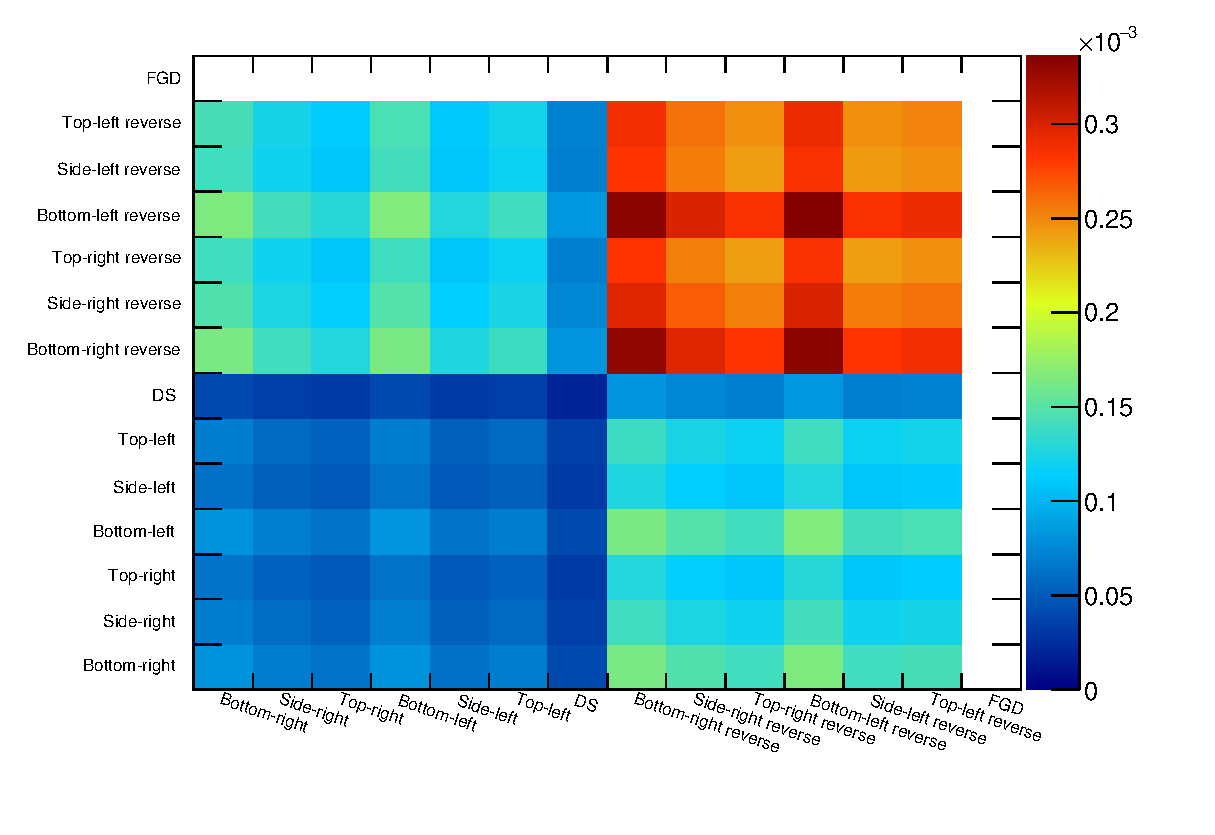
\includegraphics[width=8cm]{images/measurement/systematics/detector/oofv/ecal_oofv_covariance_matrix.eps} \label{fig:ECalOOFVShapeNormCovarianceMatrix}}
  \subfloat[Shape-only.]{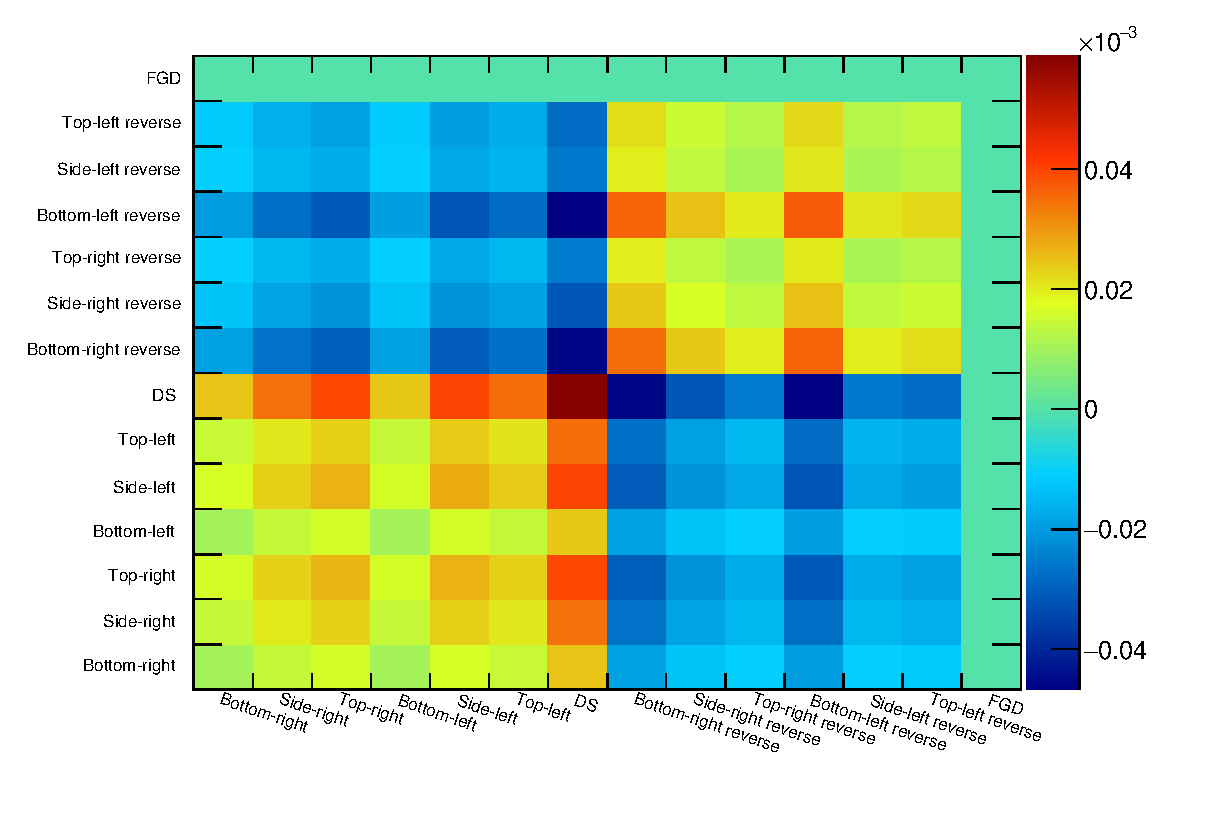
\includegraphics[width=8cm]{images/measurement/systematics/detector/oofv/ecal_oofv_shape_covariance_matrix.eps} \label{fig:ECalOOFVShapeOnlyCovarianceMatrix}}
  \caption{The sample covariance induced by the uncertainty in the ECal OOFV events.}
  \label{fig:ECalOOFVCovarianceMatrices}
\end{figure}
\newline
\newline
As described in section~\ref{sec:ReconstructionValidation}, a significant data/MC difference was found in the DS ECal reconstructed events when looking at the through-going muon control sample.  The 2D reconstructed track quality check required that tracks contained no layer gaps.  There was an unforseen hit inefficiency in the DS ECal which was not modelled in MC, which would cause tracks to be rejected because of the quality check.  This effect is shown in Fig [INSERT FIGURE].
\begin{equation}
INSERT FIGURE
\end{equation}
Because this problem was found after significant progress had been made on the MC selection, it was decided that this bug would be treated as a systematic uncertainty in the analysis.  To assess this adhoc systematic uncertainty, the quality check was relaxed to allow 2D tracks to skip one layer in a given view.  The reconstrution and selection was then applied to the sample and was compared to the nominal sample to construct the covariance matrices, which are shown in Fig.~\ref{fig:ECalHoughBugCovarianceMatrices}.
\begin{figure}%
  \centering
  \subfloat[Shape+normalisation.]{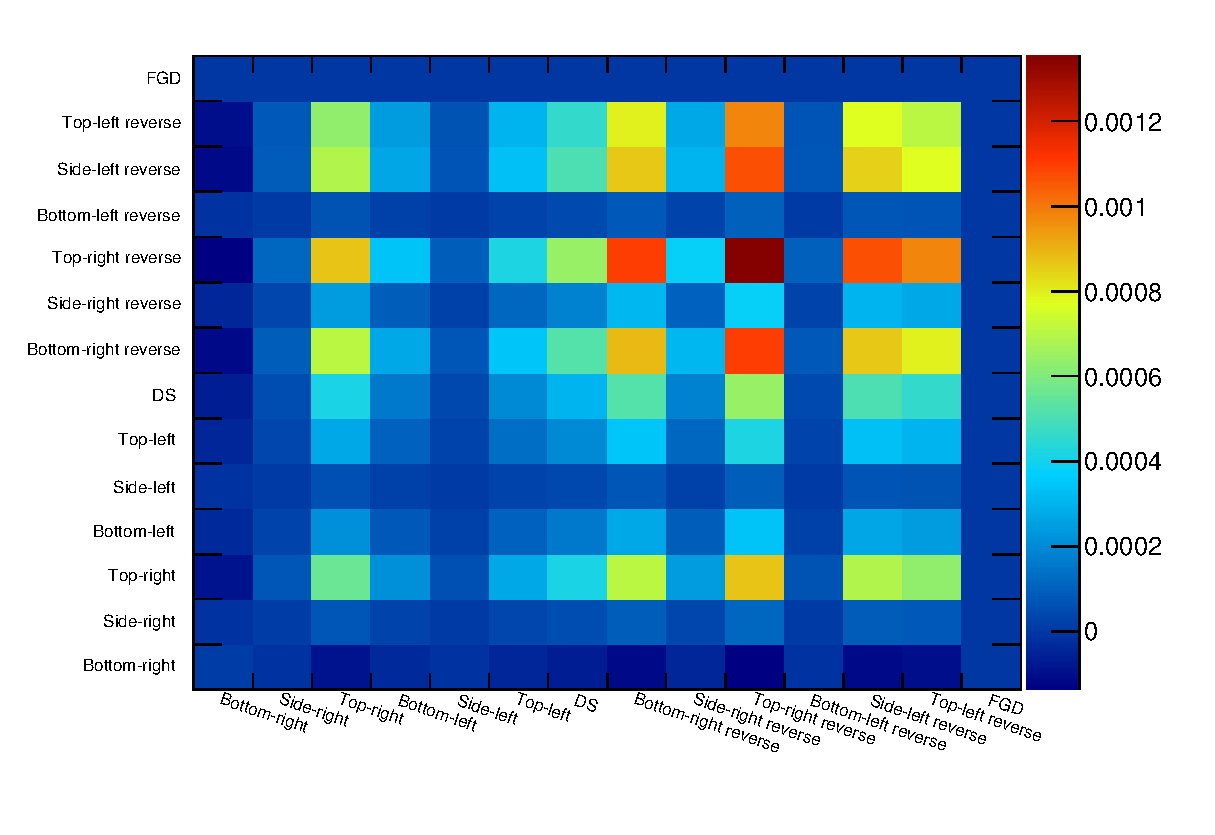
\includegraphics[width=8cm]{images/measurement/systematics/detector/bug/ecal_hough_covariance_matrix.eps} \label{fig:ECalHoughBugShapeNormCovarianceMatrix}}
  \subfloat[Shape-only.]{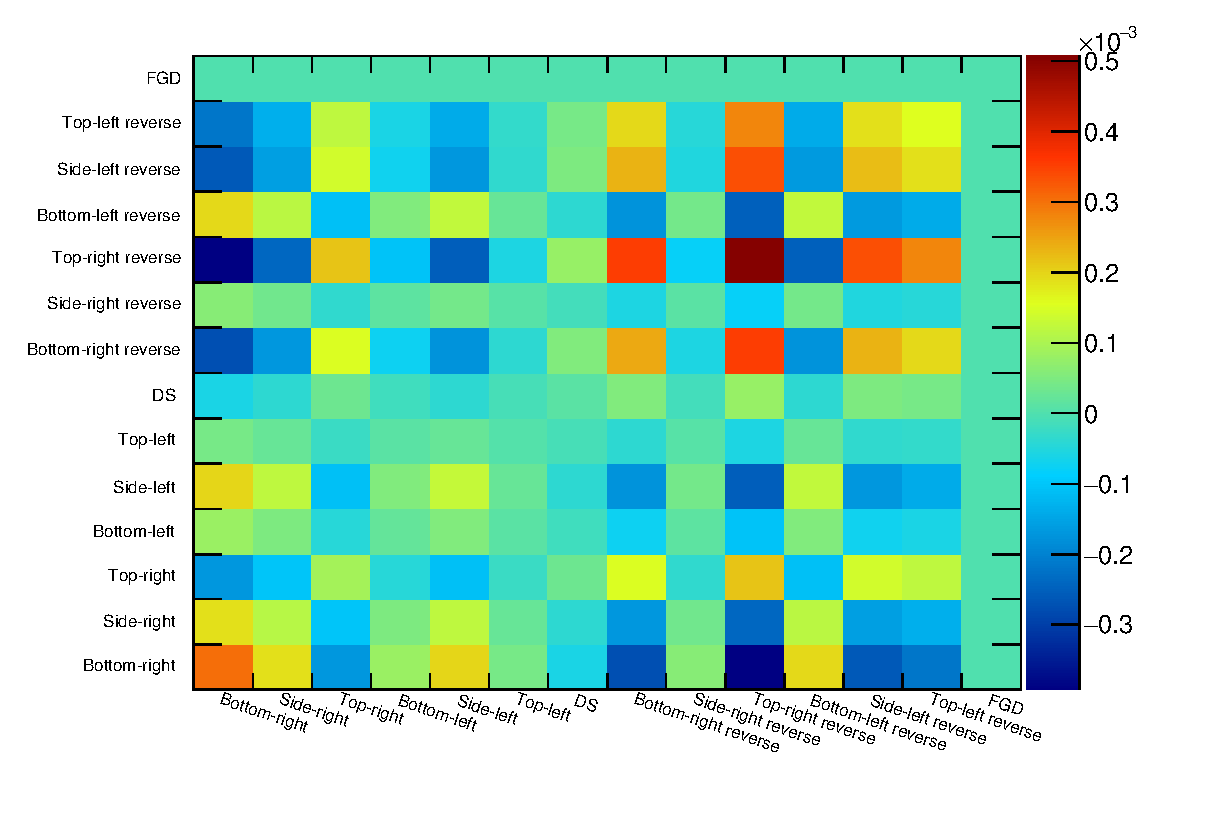
\includegraphics[width=8cm]{images/measurement/systematics/detector/bug/ecal_hough_shape_covariance_matrix.eps} \label{fig:ECalHoughBugShapeOnlyCovarianceMatrix}}
  \caption{The sample covariance induced by the bug fix to the reconstruction.}
  \label{fig:ECalHoughBugCovarianceMatrices}
\end{figure}








\section{Validation of method}
\label{sec:MethodValidation}
TESTTESTTEST
Does it work?

\section{Applying the fit to ND280 data}
\label{sec:ND280DataFit}
Run it


